\documentclass[twoside]{book}

% Packages required by doxygen
\usepackage{fixltx2e}
\usepackage{calc}
\usepackage{doxygen}
\usepackage[export]{adjustbox} % also loads graphicx
\usepackage{graphicx}
\usepackage[utf8]{inputenc}
\usepackage{makeidx}
\usepackage{multicol}
\usepackage{multirow}
\PassOptionsToPackage{warn}{textcomp}
\usepackage{textcomp}
\usepackage[nointegrals]{wasysym}
\usepackage[table]{xcolor}

% Font selection
\usepackage[T1]{fontenc}
\usepackage[scaled=.90]{helvet}
\usepackage{courier}
\usepackage{amssymb}
\usepackage{sectsty}
\renewcommand{\familydefault}{\sfdefault}
\allsectionsfont{%
  \fontseries{bc}\selectfont%
  \color{darkgray}%
}
\renewcommand{\DoxyLabelFont}{%
  \fontseries{bc}\selectfont%
  \color{darkgray}%
}
\newcommand{\+}{\discretionary{\mbox{\scriptsize$\hookleftarrow$}}{}{}}

% Page & text layout
\usepackage{geometry}
\geometry{%
  a4paper,%
  top=2.5cm,%
  bottom=2.5cm,%
  left=2.5cm,%
  right=2.5cm%
}
\tolerance=750
\hfuzz=15pt
\hbadness=750
\setlength{\emergencystretch}{15pt}
\setlength{\parindent}{0cm}
\setlength{\parskip}{3ex plus 2ex minus 2ex}
\makeatletter
\renewcommand{\paragraph}{%
  \@startsection{paragraph}{4}{0ex}{-1.0ex}{1.0ex}{%
    \normalfont\normalsize\bfseries\SS@parafont%
  }%
}
\renewcommand{\subparagraph}{%
  \@startsection{subparagraph}{5}{0ex}{-1.0ex}{1.0ex}{%
    \normalfont\normalsize\bfseries\SS@subparafont%
  }%
}
\makeatother

% Headers & footers
\usepackage{fancyhdr}
\pagestyle{fancyplain}
\fancyhead[LE]{\fancyplain{}{\bfseries\thepage}}
\fancyhead[CE]{\fancyplain{}{}}
\fancyhead[RE]{\fancyplain{}{\bfseries\leftmark}}
\fancyhead[LO]{\fancyplain{}{\bfseries\rightmark}}
\fancyhead[CO]{\fancyplain{}{}}
\fancyhead[RO]{\fancyplain{}{\bfseries\thepage}}
\fancyfoot[LE]{\fancyplain{}{}}
\fancyfoot[CE]{\fancyplain{}{}}
\fancyfoot[RE]{\fancyplain{}{\bfseries\scriptsize Generated by Doxygen }}
\fancyfoot[LO]{\fancyplain{}{\bfseries\scriptsize Generated by Doxygen }}
\fancyfoot[CO]{\fancyplain{}{}}
\fancyfoot[RO]{\fancyplain{}{}}
\renewcommand{\footrulewidth}{0.4pt}
\renewcommand{\chaptermark}[1]{%
  \markboth{#1}{}%
}
\renewcommand{\sectionmark}[1]{%
  \markright{\thesection\ #1}%
}

% Indices & bibliography
\usepackage{natbib}
\usepackage[titles]{tocloft}
\setcounter{tocdepth}{3}
\setcounter{secnumdepth}{5}
\makeindex

% Hyperlinks (required, but should be loaded last)
\usepackage{ifpdf}
\ifpdf
  \usepackage[pdftex,pagebackref=true]{hyperref}
\else
  \usepackage[ps2pdf,pagebackref=true]{hyperref}
\fi
\hypersetup{%
  colorlinks=true,%
  linkcolor=blue,%
  citecolor=blue,%
  unicode%
}

% Custom commands
\newcommand{\clearemptydoublepage}{%
  \newpage{\pagestyle{empty}\cleardoublepage}%
}

\usepackage{caption}
\captionsetup{labelsep=space,justification=centering,font={bf},singlelinecheck=off,skip=4pt,position=top}

%===== C O N T E N T S =====

\begin{document}

% Titlepage & ToC
\hypersetup{pageanchor=false,
             bookmarksnumbered=true,
             pdfencoding=unicode
            }
\pagenumbering{alph}
\begin{titlepage}
\vspace*{7cm}
\begin{center}%
{\Large Empresa de Transporte Escolar }\\
\vspace*{1cm}
{\large Generated by Doxygen 1.8.14}\\
\end{center}
\end{titlepage}
\clearemptydoublepage
\pagenumbering{roman}
\tableofcontents
\clearemptydoublepage
\pagenumbering{arabic}
\hypersetup{pageanchor=true}

%--- Begin generated contents ---
\chapter{Hierarchical Index}
\section{Class Hierarchy}
This inheritance list is sorted roughly, but not completely, alphabetically\+:\begin{DoxyCompactList}
\item \contentsline{section}{Empresa}{\pageref{class_empresa}}{}
\item \contentsline{section}{Utente}{\pageref{class_utente}}{}
\begin{DoxyCompactList}
\item \contentsline{section}{Crianca}{\pageref{class_crianca}}{}
\item \contentsline{section}{Funcionario}{\pageref{class_funcionario}}{}
\end{DoxyCompactList}
\item \contentsline{section}{Veiculo}{\pageref{class_veiculo}}{}
\begin{DoxyCompactList}
\item \contentsline{section}{Escolar}{\pageref{class_escolar}}{}
\item \contentsline{section}{Recreativo}{\pageref{class_recreativo}}{}
\end{DoxyCompactList}
\end{DoxyCompactList}

\chapter{Class Index}
\section{Class List}
Here are the classes, structs, unions and interfaces with brief descriptions\+:\begin{DoxyCompactList}
\item\contentsline{section}{\mbox{\hyperlink{class_crianca}{Crianca}} \\*Classe para instanciar criancas }{\pageref{class_crianca}}{}
\item\contentsline{section}{\mbox{\hyperlink{class_empresa}{Empresa}} \\*Classe que representa uma empresa de transportes }{\pageref{class_empresa}}{}
\item\contentsline{section}{\mbox{\hyperlink{class_escolar}{Escolar}} \\*Classe para instanciar transportes escolares }{\pageref{class_escolar}}{}
\item\contentsline{section}{\mbox{\hyperlink{class_funcionario}{Funcionario}} \\*Classe para instanciar funcionarios }{\pageref{class_funcionario}}{}
\item\contentsline{section}{\mbox{\hyperlink{class_recreativo}{Recreativo}} \\*Classe para instanciar transportes de atividades recreativas }{\pageref{class_recreativo}}{}
\item\contentsline{section}{\mbox{\hyperlink{class_utente}{Utente}} \\*Classe para instanciar utentes }{\pageref{class_utente}}{}
\item\contentsline{section}{\mbox{\hyperlink{class_veiculo}{Veiculo}} \\*Classe para instanciar veiculos }{\pageref{class_veiculo}}{}
\end{DoxyCompactList}

\chapter{Class Documentation}
\hypertarget{class_crianca}{}\section{Crianca Class Reference}
\label{class_crianca}\index{Crianca@{Crianca}}


Classe para instanciar criancas.  




{\ttfamily \#include $<$Utente.\+h$>$}

Inheritance diagram for Crianca\+:\begin{figure}[H]
\begin{center}
\leavevmode
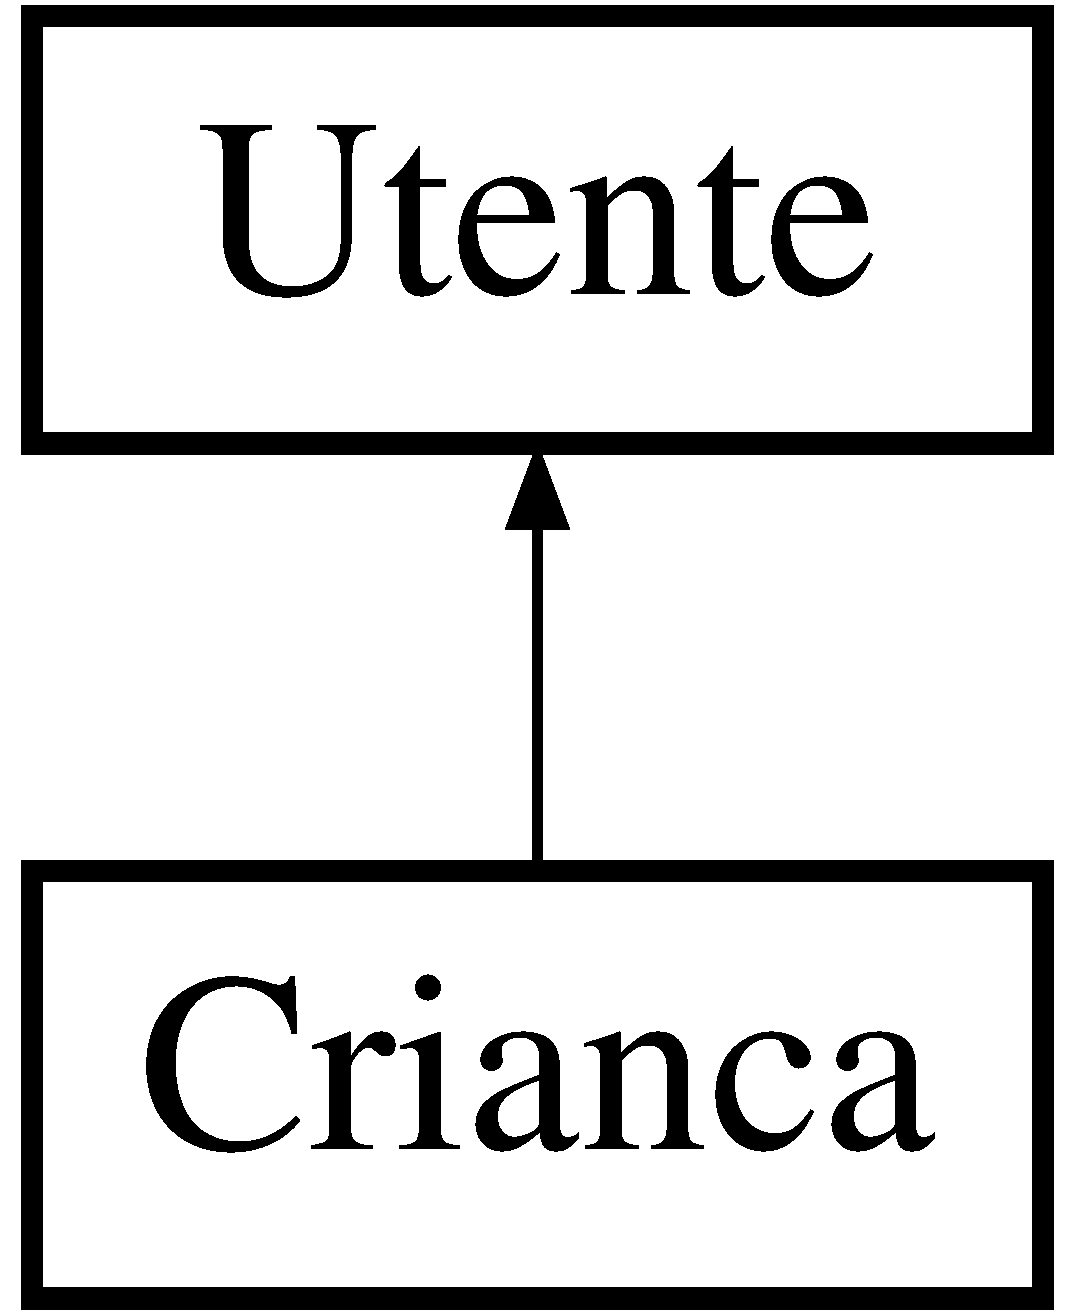
\includegraphics[height=2.000000cm]{class_crianca}
\end{center}
\end{figure}
\subsection*{Public Member Functions}
\begin{DoxyCompactItemize}
\item 
\mbox{\hyperlink{class_crianca_a3b66bc9f3d1302400f5fec96f380f669}{Crianca}} (const string \&\mbox{\hyperlink{class_utente_a328c722d27759eaa88596ccb4cf2549f}{nome}}, const string \&data\+\_\+nasc, const string \&\mbox{\hyperlink{class_utente_ac5acf8e42ccd10808d077fc0db2e05f9}{BI}}, const unsigned int \&zona\+Habit, const unsigned int \&zona\+Esc, const string \&nome\+EE, const unsigned int \&contacto\+EE)
\begin{DoxyCompactList}\small\item\em Construtor da classe \mbox{\hyperlink{class_crianca}{Crianca}}. \end{DoxyCompactList}\item 
string \mbox{\hyperlink{class_crianca_ab93207d112d82437a86b230e1e0a5835}{get\+Nome\+EE}} () const
\begin{DoxyCompactList}\small\item\em Permite acesso ao nome do Encarregado de Educacao da crianca. \end{DoxyCompactList}\item 
unsigned int \mbox{\hyperlink{class_crianca_a528589e1353aa4eb4348e9e1d67b6a47}{get\+Contacto}} () const
\begin{DoxyCompactList}\small\item\em Permite acesso ao contacto do Encarregado de Educacao da crianca. \end{DoxyCompactList}\item 
void \mbox{\hyperlink{class_crianca_ac5a08589414697db0269fbcf44bb96f0}{set\+Contacto}} (unsigned int cont)
\begin{DoxyCompactList}\small\item\em Altera o contacto do Encarregado de Educacao da crianca. \end{DoxyCompactList}\item 
string \mbox{\hyperlink{class_crianca_a7cd065415f6f0a2802ca2d37a3a7cc25}{get\+Info}} () const
\begin{DoxyCompactList}\small\item\em Organiza a informacao da crianca para ser guardada em ficheiro. \end{DoxyCompactList}\end{DoxyCompactItemize}
\subsection*{Friends}
\begin{DoxyCompactItemize}
\item 
\mbox{\Hypertarget{class_crianca_a2a82fda6331ef8d7e44a861ec86a5a6e}\label{class_crianca_a2a82fda6331ef8d7e44a861ec86a5a6e}} 
ostream \& {\bfseries operator$<$$<$} (ostream \&out, const \mbox{\hyperlink{class_crianca}{Crianca}} \&utente)
\end{DoxyCompactItemize}
\subsection*{Additional Inherited Members}


\subsection{Detailed Description}
Classe para instanciar criancas. 

Para alem das caracteristicas de um utente normal, a crianca tem associados o nome do Encarregado de Educacao e o contacto deste. 

\subsection{Constructor \& Destructor Documentation}
\mbox{\Hypertarget{class_crianca_a3b66bc9f3d1302400f5fec96f380f669}\label{class_crianca_a3b66bc9f3d1302400f5fec96f380f669}} 
\index{Crianca@{Crianca}!Crianca@{Crianca}}
\index{Crianca@{Crianca}!Crianca@{Crianca}}
\subsubsection{\texorpdfstring{Crianca()}{Crianca()}}
{\footnotesize\ttfamily Crianca\+::\+Crianca (\begin{DoxyParamCaption}\item[{const string \&}]{nome,  }\item[{const string \&}]{data\+\_\+nasc,  }\item[{const string \&}]{BI,  }\item[{const unsigned int \&}]{zona\+Habit,  }\item[{const unsigned int \&}]{zona\+Esc,  }\item[{const string \&}]{nome\+EE,  }\item[{const unsigned int \&}]{contacto\+EE }\end{DoxyParamCaption})}



Construtor da classe \mbox{\hyperlink{class_crianca}{Crianca}}. 


\begin{DoxyParams}{Parameters}
{\em nome} & Nome da crianca \\
\hline
{\em data\+\_\+nasc} & Data de nascimento \\
\hline
{\em BI} & BI da crianca \\
\hline
{\em zona\+Habit} & Zona de habitacao da crianca \\
\hline
{\em zona\+Esc} & Zona da escola da crianca \\
\hline
{\em nome\+EE} & Nome do Encarregado de Educacao \\
\hline
{\em contacto\+EE} & Contacto do Encarregado de Educacao \\
\hline
\end{DoxyParams}


\subsection{Member Function Documentation}
\mbox{\Hypertarget{class_crianca_a528589e1353aa4eb4348e9e1d67b6a47}\label{class_crianca_a528589e1353aa4eb4348e9e1d67b6a47}} 
\index{Crianca@{Crianca}!get\+Contacto@{get\+Contacto}}
\index{get\+Contacto@{get\+Contacto}!Crianca@{Crianca}}
\subsubsection{\texorpdfstring{get\+Contacto()}{getContacto()}}
{\footnotesize\ttfamily unsigned int Crianca\+::get\+Contacto (\begin{DoxyParamCaption}{ }\end{DoxyParamCaption}) const\hspace{0.3cm}{\ttfamily [virtual]}}



Permite acesso ao contacto do Encarregado de Educacao da crianca. 

\begin{DoxyReturn}{Returns}
contacto do encarregado de educacao (unsigned int) 
\end{DoxyReturn}


Implements \mbox{\hyperlink{class_utente}{Utente}}.

\mbox{\Hypertarget{class_crianca_a7cd065415f6f0a2802ca2d37a3a7cc25}\label{class_crianca_a7cd065415f6f0a2802ca2d37a3a7cc25}} 
\index{Crianca@{Crianca}!get\+Info@{get\+Info}}
\index{get\+Info@{get\+Info}!Crianca@{Crianca}}
\subsubsection{\texorpdfstring{get\+Info()}{getInfo()}}
{\footnotesize\ttfamily string Crianca\+::get\+Info (\begin{DoxyParamCaption}{ }\end{DoxyParamCaption}) const\hspace{0.3cm}{\ttfamily [virtual]}}



Organiza a informacao da crianca para ser guardada em ficheiro. 

\begin{DoxyReturn}{Returns}
string com toda a informacao da crianca (atributos separados por tabs) 
\end{DoxyReturn}


Reimplemented from \mbox{\hyperlink{class_utente_aee03eae2a7154e7b4713b2be195d548f}{Utente}}.

\mbox{\Hypertarget{class_crianca_ab93207d112d82437a86b230e1e0a5835}\label{class_crianca_ab93207d112d82437a86b230e1e0a5835}} 
\index{Crianca@{Crianca}!get\+Nome\+EE@{get\+Nome\+EE}}
\index{get\+Nome\+EE@{get\+Nome\+EE}!Crianca@{Crianca}}
\subsubsection{\texorpdfstring{get\+Nome\+E\+E()}{getNomeEE()}}
{\footnotesize\ttfamily string Crianca\+::get\+Nome\+EE (\begin{DoxyParamCaption}{ }\end{DoxyParamCaption}) const\hspace{0.3cm}{\ttfamily [virtual]}}



Permite acesso ao nome do Encarregado de Educacao da crianca. 

\begin{DoxyReturn}{Returns}
string com o nome do encarregado de educacao 
\end{DoxyReturn}


Reimplemented from \mbox{\hyperlink{class_utente}{Utente}}.

\mbox{\Hypertarget{class_crianca_ac5a08589414697db0269fbcf44bb96f0}\label{class_crianca_ac5a08589414697db0269fbcf44bb96f0}} 
\index{Crianca@{Crianca}!set\+Contacto@{set\+Contacto}}
\index{set\+Contacto@{set\+Contacto}!Crianca@{Crianca}}
\subsubsection{\texorpdfstring{set\+Contacto()}{setContacto()}}
{\footnotesize\ttfamily void Crianca\+::set\+Contacto (\begin{DoxyParamCaption}\item[{unsigned int}]{cont }\end{DoxyParamCaption})\hspace{0.3cm}{\ttfamily [virtual]}}



Altera o contacto do Encarregado de Educacao da crianca. 


\begin{DoxyParams}{Parameters}
{\em cont} & Novo contacto do Encarregado de Educacao \\
\hline
\end{DoxyParams}


Implements \mbox{\hyperlink{class_utente}{Utente}}.



The documentation for this class was generated from the following files\+:\begin{DoxyCompactItemize}
\item 
C\+:/\+Users/\+Cajo/\+Desktop/\+Repos/\+A\+E\+D\+A-\/\+P\+R\+O\+J1/src/Utente.\+h\item 
C\+:/\+Users/\+Cajo/\+Desktop/\+Repos/\+A\+E\+D\+A-\/\+P\+R\+O\+J1/src/Utente.\+cpp\end{DoxyCompactItemize}

\hypertarget{class_empresa}{}\section{Empresa Class Reference}
\label{class_empresa}\index{Empresa@{Empresa}}


Classe que representa uma empresa de transportes.  




{\ttfamily \#include $<$Empresa\+Transportes.\+h$>$}

\subsection*{Public Member Functions}
\begin{DoxyCompactItemize}
\item 
\mbox{\hyperlink{class_empresa_ac5bccaf3758b25fea4803a63d4362236}{Empresa}} (string nome)
\begin{DoxyCompactList}\small\item\em Construtor simples da classe \mbox{\hyperlink{class_empresa}{Empresa}} Usado para criar uma \mbox{\hyperlink{class_empresa}{Empresa}} de raiz. \end{DoxyCompactList}\item 
\mbox{\hyperlink{class_empresa_a3eabce52f65fae491d7b3dc28d6eb6e5}{Empresa}} (ifstream \&f)
\begin{DoxyCompactList}\small\item\em Construtor a partir de ficheiro da classe \mbox{\hyperlink{class_empresa}{Empresa}} Usado para carregar uma \mbox{\hyperlink{class_empresa}{Empresa}} previamente gravado num ficheiro. \end{DoxyCompactList}\item 
\mbox{\hyperlink{class_empresa_a093f61d3da9863f22291e02cbaed05e7}{Empresa}} (string nome, vector$<$ \mbox{\hyperlink{class_utente}{Utente}} $\ast$$>$ v\+Ut, vector$<$ \mbox{\hyperlink{class_veiculo}{Veiculo}} $\ast$$>$ v\+Veic, unsigned int preco\+Pessoa, ifstream \&fprecos)
\begin{DoxyCompactList}\small\item\em Construtor completo da classe \mbox{\hyperlink{class_empresa}{Empresa}}. \end{DoxyCompactList}\item 
string \mbox{\hyperlink{class_empresa_af18ca7018ca4771c59ee3b36bc6c213b}{get\+Nome}} () const
\begin{DoxyCompactList}\small\item\em Permite acesso ao nome da empresa. \end{DoxyCompactList}\item 
vector$<$ \mbox{\hyperlink{class_veiculo}{Veiculo}} $\ast$ $>$ \mbox{\hyperlink{class_empresa_a64b4f5f7e313a07569451b5a82f822bb}{get\+Veiculos}} () const
\begin{DoxyCompactList}\small\item\em Permite acesso a listagem de veiculos da empresa. \end{DoxyCompactList}\item 
vector$<$ \mbox{\hyperlink{class_utente}{Utente}} $\ast$ $>$ \mbox{\hyperlink{class_empresa_a8eded445f1ae7289bb1ba77adb7c581e}{get\+Utentes}} () const
\begin{DoxyCompactList}\small\item\em Permite acesso a listagem de utentes da empresa. \end{DoxyCompactList}\item 
unsigned int \mbox{\hyperlink{class_empresa_a0c2b8d30106124c1eb34e82769337656}{get\+Preco\+Pessoa}} () const
\begin{DoxyCompactList}\small\item\em Permite acesso ao preco de aluguer por pessoa definido pela empresa. \end{DoxyCompactList}\item 
vector$<$ vector$<$ double $>$ $>$ \mbox{\hyperlink{class_empresa_a1b5f74cd32b847b36d39bba103e34f24}{get\+Precos}} () const
\begin{DoxyCompactList}\small\item\em Permite acesso a matrix de precos de passes por zona usada na empresa. \end{DoxyCompactList}\item 
void \mbox{\hyperlink{class_empresa_a0733c7676b94e4e273b3e9b5f7d1c5ad}{set\+Utentes}} (vector$<$ \mbox{\hyperlink{class_utente}{Utente}} $\ast$$>$ v\+Ut)
\begin{DoxyCompactList}\small\item\em Altera a listagem de utentes da empresa para uma nova. \end{DoxyCompactList}\item 
void \mbox{\hyperlink{class_empresa_a6e492b399a9e3362ed1b50fb05bb36b5}{set\+Veiculos}} (vector$<$ \mbox{\hyperlink{class_veiculo}{Veiculo}} $\ast$$>$ v\+Veic)
\begin{DoxyCompactList}\small\item\em Altera a listagem de veiculos da empresa para uma nova. \end{DoxyCompactList}\item 
void \mbox{\hyperlink{class_empresa_aa2ecc54f025070f55e013dd439c22936}{set\+Preco\+Pessoa}} (unsigned int precoP)
\begin{DoxyCompactList}\small\item\em Altera o preco de aluguer por pessoa. \end{DoxyCompactList}\item 
void \mbox{\hyperlink{class_empresa_aad5017fad374ed1cc8f25016cc5b4eb5}{set\+Precos}} (istream \&fprecos)
\begin{DoxyCompactList}\small\item\em Carrega de um ficheiro a matriz de precos dos passes. \end{DoxyCompactList}\item 
void \mbox{\hyperlink{class_empresa_a5045b1da6fe55685e04a89d4fd61aa1a}{set\+Precos}} (const vector$<$ vector$<$ double $>$$>$ \&vet)
\begin{DoxyCompactList}\small\item\em Altera a matriz de precos empresa para uma nova. \end{DoxyCompactList}\item 
void \mbox{\hyperlink{class_empresa_abe88713c8f7666b9ae119700fc318d78}{adicionar\+Veiculo}} (\mbox{\hyperlink{class_veiculo}{Veiculo}} $\ast$vc)
\begin{DoxyCompactList}\small\item\em Adiciona um \mbox{\hyperlink{class_veiculo}{Veiculo}} a listagem ja existente na empresa. \end{DoxyCompactList}\item 
void \mbox{\hyperlink{class_empresa_ae2ff321878007fa832020aab9991dba0}{adicionar\+Utente}} (\mbox{\hyperlink{class_utente}{Utente}} $\ast$ut)
\begin{DoxyCompactList}\small\item\em Adiciona um \mbox{\hyperlink{class_utente}{Utente}} a listagem ja existente na empresa. \end{DoxyCompactList}\item 
void \mbox{\hyperlink{class_empresa_a345839f16710bfd88e3a5fbcf14a3909}{remover\+Veiculo}} (unsigned int id)
\begin{DoxyCompactList}\small\item\em Remove o \mbox{\hyperlink{class_veiculo}{Veiculo}} especificado da listagem ja existente na empresa. \end{DoxyCompactList}\item 
void \mbox{\hyperlink{class_empresa_a39f49199e53094afe62e3d4150121f6b}{remover\+Veiculo}} (string matricula)
\begin{DoxyCompactList}\small\item\em Remove o \mbox{\hyperlink{class_veiculo}{Veiculo}} especificado da listagem ja existente na empresa. \end{DoxyCompactList}\item 
void \mbox{\hyperlink{class_empresa_a216c65bc97b0f205537f914c3171584c}{remover\+Utente}} (unsigned int num\+Ut)
\begin{DoxyCompactList}\small\item\em Remove o \mbox{\hyperlink{class_utente}{Utente}} especificado da listagem ja existente na empresa. \end{DoxyCompactList}\item 
void \mbox{\hyperlink{class_empresa_a3550486deddb6eea8a94aa25fb4c5f37}{remover\+Utente}} (string BI)
\begin{DoxyCompactList}\small\item\em Remove o \mbox{\hyperlink{class_utente}{Utente}} especificado da listagem ja existente na empresa. \end{DoxyCompactList}\item 
void \mbox{\hyperlink{class_empresa_a09c03bb10c301da04287107a1fcfd63e}{adicionar\+Zona\+Escolar}} (unsigned int idV, unsigned int zona)
\begin{DoxyCompactList}\small\item\em Adiciona ao transporte escolar especificaddo uma zona. \end{DoxyCompactList}\item 
void \mbox{\hyperlink{class_empresa_a2f3365974dff2a149c1818f9d6783deb}{remover\+Zona\+Escolar}} (unsigned int idV, unsigned int zona)
\begin{DoxyCompactList}\small\item\em Remove do transporte escolar especificaddo uma zona. \end{DoxyCompactList}\item 
void \mbox{\hyperlink{class_empresa_a90633274606d1983946d53523ed3eaa4}{alterar\+Zona\+Hab}} (unsigned int num\+Utente, unsigned int zona)
\begin{DoxyCompactList}\small\item\em Modifica a zona de habitacao do utente especificado. \end{DoxyCompactList}\item 
void \mbox{\hyperlink{class_empresa_a87c4477cee0f0889942804ba69dd0791}{alterar\+Zona\+Esc}} (unsigned int num\+Utente, unsigned int zona)
\begin{DoxyCompactList}\small\item\em Modifica a zona da escola do utente especificado. \end{DoxyCompactList}\item 
void \mbox{\hyperlink{class_empresa_acde85d7276904f10937a41f60060cd67}{alterar\+Contacto}} (unsigned int num\+Utente, unsigned int cont)
\begin{DoxyCompactList}\small\item\em Substitui o contacto do utente especificado Caso o utente seja um funcinario substitui o seu contacto, caso seja crianca substitui o contacto do Encarregado de Educacao. \end{DoxyCompactList}\item 
unsigned int \mbox{\hyperlink{class_empresa_ae2d2c99704126f1364b666f1973fb8cf}{get\+Contacto}} (unsigned int num\+Utente)
\begin{DoxyCompactList}\small\item\em Devolve o contacto do utente especificado Caso o utente seja um funcinario devolve o seu contacto, caso seja crianca devolve o contacto do Encarregado de Educacao. \end{DoxyCompactList}\item 
unsigned int \mbox{\hyperlink{class_empresa_aef73b3ec5119615f092a71a149c7f9eb}{get\+Contacto}} (string BI)
\begin{DoxyCompactList}\small\item\em Devolve o contacto do utente especificado Caso o utente seja um funcinario devolve o seu contacto, caso seja crianca devolve o contacto do Encarregado de Educacao. \end{DoxyCompactList}\item 
double \mbox{\hyperlink{class_empresa_a1fceee003267c33641d908f4b3d4d3f2}{calculo\+Passe\+Mensal}} (unsigned int num\+Utente)
\begin{DoxyCompactList}\small\item\em Calcula o valor do passe mensal do utente especificado Determina quais as zonas de habitacao e de escola do utente e usa-\/as para aceder a matrix de precos e devolver o valor do passe. \end{DoxyCompactList}\item 
\mbox{\Hypertarget{class_empresa_aad0a7204589c3ef5ff4ef9bf7e61819e}\label{class_empresa_aad0a7204589c3ef5ff4ef9bf7e61819e}} 
void \mbox{\hyperlink{class_empresa_aad0a7204589c3ef5ff4ef9bf7e61819e}{atualizar\+Passes}} ()
\begin{DoxyCompactList}\small\item\em Estabelece a correspondecia entre todos os utentes e os valores dos passes mensais Recorre ao metodo \mbox{\hyperlink{class_empresa_a1fceee003267c33641d908f4b3d4d3f2}{calculo\+Passe\+Mensal()}} para calcular individualmente o valor do passe para cada utente e guarda essa correspondencia na tabela\+Passes. \end{DoxyCompactList}\item 
void \mbox{\hyperlink{class_empresa_aa2d2b0e64413e2ddf6c29c82daa5a743}{atualizar\+Precos}} (double delta)
\begin{DoxyCompactList}\small\item\em Atualiza todos os precos na matrix de precos por zona. \end{DoxyCompactList}\item 
double \mbox{\hyperlink{class_empresa_a1aeac933b91a2abfb92d11ba51fe3699}{calcular\+Aluguer}} (unsigned int idV)
\begin{DoxyCompactList}\small\item\em Calcula o preco do aluguer do transporte recreativo especificado. Baseia-\/se no preco de aluguer por pessoa e na capcidade do veiculo para fazer o calculo. \end{DoxyCompactList}\item 
string \mbox{\hyperlink{class_empresa_a36bb8eb5b7825df35e30164fd74e508e}{verifica\+Disp\+Recreativo}} (unsigned int capacidade)
\begin{DoxyCompactList}\small\item\em Verifica quais os transportes recreativos disponiveis para alugar. Devolve informacao relativa a todos os recreativos disponiveis (Id, Capacidade, Preco). \end{DoxyCompactList}\item 
void \mbox{\hyperlink{class_empresa_a07dc1066c3bbe1e1043f3d0f3004645c}{aluga\+Recreativo}} (unsigned int idV)
\begin{DoxyCompactList}\small\item\em Aluga o trasnporte recreativo especificado por um dia. \end{DoxyCompactList}\item 
\mbox{\Hypertarget{class_empresa_a90c7dfc23aba2ddead3c72ed39bc843f}\label{class_empresa_a90c7dfc23aba2ddead3c72ed39bc843f}} 
void \mbox{\hyperlink{class_empresa_a90c7dfc23aba2ddead3c72ed39bc843f}{aloca\+Utentes}} ()
\begin{DoxyCompactList}\small\item\em Processa a alocacao de passageiros para os transportes escolares. A cada utente faz corresponder o veiculo (sempre um transporte escolar) que tem de usar. Nao o faz com nenhum criterio especifico, apenas vai por ordem crescente de numero de identificacao de utente e de veiculo O resultado da alocacao e uma tabela de corresnpondencias entre Utentes e Veiculos, i.\+e. a tabela\+Passageiros Se nao existirem veiculos suficientes para todos os utentes lanca uma excecao do tipo Veiculos\+Insuficientes. \end{DoxyCompactList}\item 
void \mbox{\hyperlink{class_empresa_a01d9d82ed48240d69fcb99f82f4ff404}{aloca\+Ut}} (unsigned int num\+Ut)
\begin{DoxyCompactList}\small\item\em Aloca apenas o utente especificado a um transporte escolar O resultado da alocacao e guardado na tabela\+Passageiros. \end{DoxyCompactList}\item 
bool \mbox{\hyperlink{class_empresa_af41234653cd92b527030ebd3f67ee7a5}{final\+Dia}} (float kms\+Zona)
\begin{DoxyCompactList}\small\item\em Processa o final de um dia na empresa Calcula todos os gastos de todos os veiculos, bem como os ganhos com o aluguer de recreativos e guarda a informacao sobre o balanco do dia no vetor registo\+Diario. Para alem disso, todos os trasnportes recreativos alugados passam a estar livres para o dia seguinte, dando assim inicio a um novo dia. \end{DoxyCompactList}\item 
bool \mbox{\hyperlink{class_empresa_a4a1e541280c5f7ae9e3f418d33b4cbd2}{calculo\+Mensal}} ()
\begin{DoxyCompactList}\small\item\em Processa o calculo do lucro mensal na empresa Tendo em conta os balancos diarios e os valores dos passes mensais, calcula o lucro tirado no final do mes, dando assim inicio a um novo mes. Os lucros sao guardados no vetor lucros\+Mensais e quando se insere o 12o valor a funcao da inicio a um novo ano civil. \end{DoxyCompactList}\item 
void \mbox{\hyperlink{class_empresa_a4bfb65fa408e944aed798e7c37933b78}{guardar\+Info}} (ostream \&f) const
\begin{DoxyCompactList}\small\item\em Envia toda a informacao da empresa para a ostream especificada. Usando um ficheiro, a funcao guarda a informacao nesse ficheiro. \end{DoxyCompactList}\item 
void \mbox{\hyperlink{class_empresa_a3561dcd8cfee00b63e7fd48207c7831f}{carregar\+Info}} (ifstream \&f)
\begin{DoxyCompactList}\small\item\em Carrega toda a informacao da empresa a partir de um ficheiro de texto. \end{DoxyCompactList}\item 
string \mbox{\hyperlink{class_empresa_acd94b5de5f758663768d4c4af41b0039}{show\+Utentes}} () const
\begin{DoxyCompactList}\small\item\em Devolve a informacao dos utentes da empresa. \end{DoxyCompactList}\item 
string \mbox{\hyperlink{class_empresa_a5a6d0c8a801a77a5bf48e32a96890c61}{show\+Veiculos}} () const
\begin{DoxyCompactList}\small\item\em Devolve informacao dos veiculos da empresa. \end{DoxyCompactList}\item 
string \mbox{\hyperlink{class_empresa_a3dbd5fca995d27f9911d5e694e01c76e}{show\+Mensal}} () const
\begin{DoxyCompactList}\small\item\em Devolve a informacao dos lucros mensais da empresa. \end{DoxyCompactList}\item 
string \mbox{\hyperlink{class_empresa_a3c7180cf55b876478c0774055f2cfd31}{show\+Diario}} () const
\begin{DoxyCompactList}\small\item\em Devolve a informacao dos balancos diarios da empresa. \end{DoxyCompactList}\end{DoxyCompactItemize}
\subsection*{Friends}
\begin{DoxyCompactItemize}
\item 
\mbox{\Hypertarget{class_empresa_a112287fd62f96ae691f61dae056dcd79}\label{class_empresa_a112287fd62f96ae691f61dae056dcd79}} 
ostream \& {\bfseries operator$<$$<$} (ostream \&out, const \mbox{\hyperlink{class_empresa}{Empresa}} \&emp)
\end{DoxyCompactItemize}


\subsection{Detailed Description}
Classe que representa uma empresa de transportes. 

A classe reune algumas informacoes importantes sobre a empresa, tais como o seu nome, a frota de veiculos, a lista de utentes e os lucros obtidos. Permite gerir o que acontece na empresa atraves de variadissimos metodos que fornecem as abstracoes necessarias para proporcionar uma gestao intuitiva e simples. Todas as informacoes da empresa podem ser guardadas em ficeiro de texo para mais tarde serem carregadas e alteradas como necessario. 

\subsection{Constructor \& Destructor Documentation}
\mbox{\Hypertarget{class_empresa_ac5bccaf3758b25fea4803a63d4362236}\label{class_empresa_ac5bccaf3758b25fea4803a63d4362236}} 
\index{Empresa@{Empresa}!Empresa@{Empresa}}
\index{Empresa@{Empresa}!Empresa@{Empresa}}
\subsubsection{\texorpdfstring{Empresa()}{Empresa()}\hspace{0.1cm}{\footnotesize\ttfamily [1/3]}}
{\footnotesize\ttfamily Empresa\+::\+Empresa (\begin{DoxyParamCaption}\item[{string}]{nome }\end{DoxyParamCaption})}



Construtor simples da classe \mbox{\hyperlink{class_empresa}{Empresa}} Usado para criar uma \mbox{\hyperlink{class_empresa}{Empresa}} de raiz. 


\begin{DoxyParams}{Parameters}
{\em nome} & Nome da empresa \\
\hline
\end{DoxyParams}
\mbox{\Hypertarget{class_empresa_a3eabce52f65fae491d7b3dc28d6eb6e5}\label{class_empresa_a3eabce52f65fae491d7b3dc28d6eb6e5}} 
\index{Empresa@{Empresa}!Empresa@{Empresa}}
\index{Empresa@{Empresa}!Empresa@{Empresa}}
\subsubsection{\texorpdfstring{Empresa()}{Empresa()}\hspace{0.1cm}{\footnotesize\ttfamily [2/3]}}
{\footnotesize\ttfamily Empresa\+::\+Empresa (\begin{DoxyParamCaption}\item[{ifstream \&}]{f }\end{DoxyParamCaption})}



Construtor a partir de ficheiro da classe \mbox{\hyperlink{class_empresa}{Empresa}} Usado para carregar uma \mbox{\hyperlink{class_empresa}{Empresa}} previamente gravado num ficheiro. 


\begin{DoxyParams}{Parameters}
{\em f} & Ficheiro de texto em que se encontra um empresa guardada \\
\hline
\end{DoxyParams}
\mbox{\Hypertarget{class_empresa_a093f61d3da9863f22291e02cbaed05e7}\label{class_empresa_a093f61d3da9863f22291e02cbaed05e7}} 
\index{Empresa@{Empresa}!Empresa@{Empresa}}
\index{Empresa@{Empresa}!Empresa@{Empresa}}
\subsubsection{\texorpdfstring{Empresa()}{Empresa()}\hspace{0.1cm}{\footnotesize\ttfamily [3/3]}}
{\footnotesize\ttfamily Empresa\+::\+Empresa (\begin{DoxyParamCaption}\item[{string}]{nome,  }\item[{vector$<$ \mbox{\hyperlink{class_utente}{Utente}} $\ast$$>$}]{v\+Ut,  }\item[{vector$<$ \mbox{\hyperlink{class_veiculo}{Veiculo}} $\ast$$>$}]{v\+Veic,  }\item[{unsigned int}]{preco\+Pessoa,  }\item[{ifstream \&}]{fprecos }\end{DoxyParamCaption})}



Construtor completo da classe \mbox{\hyperlink{class_empresa}{Empresa}}. 


\begin{DoxyParams}{Parameters}
{\em nome} & Nome da empresa \\
\hline
{\em v\+Ut} & Vetor de utentes da empresa \\
\hline
{\em v\+Veic} & Vetor de veiculos da empresa \\
\hline
{\em preco\+Pessoa} & Valor do preco do aluguer por pessoa \\
\hline
{\em fprecos} & Ficheiro contendo a matrix de precos dos passes a ser carregada \\
\hline
\end{DoxyParams}


\subsection{Member Function Documentation}
\mbox{\Hypertarget{class_empresa_ae2ff321878007fa832020aab9991dba0}\label{class_empresa_ae2ff321878007fa832020aab9991dba0}} 
\index{Empresa@{Empresa}!adicionar\+Utente@{adicionar\+Utente}}
\index{adicionar\+Utente@{adicionar\+Utente}!Empresa@{Empresa}}
\subsubsection{\texorpdfstring{adicionar\+Utente()}{adicionarUtente()}}
{\footnotesize\ttfamily void Empresa\+::adicionar\+Utente (\begin{DoxyParamCaption}\item[{\mbox{\hyperlink{class_utente}{Utente}} $\ast$}]{ut }\end{DoxyParamCaption})}



Adiciona um \mbox{\hyperlink{class_utente}{Utente}} a listagem ja existente na empresa. 


\begin{DoxyParams}{Parameters}
{\em ut} & \mbox{\hyperlink{class_utente}{Utente}} a ser adicionado\\
\hline
\end{DoxyParams}
Se o utente ja existir lanca uma excecao do tipo Utente\+Ja\+Existe \mbox{\Hypertarget{class_empresa_abe88713c8f7666b9ae119700fc318d78}\label{class_empresa_abe88713c8f7666b9ae119700fc318d78}} 
\index{Empresa@{Empresa}!adicionar\+Veiculo@{adicionar\+Veiculo}}
\index{adicionar\+Veiculo@{adicionar\+Veiculo}!Empresa@{Empresa}}
\subsubsection{\texorpdfstring{adicionar\+Veiculo()}{adicionarVeiculo()}}
{\footnotesize\ttfamily void Empresa\+::adicionar\+Veiculo (\begin{DoxyParamCaption}\item[{\mbox{\hyperlink{class_veiculo}{Veiculo}} $\ast$}]{vc }\end{DoxyParamCaption})}



Adiciona um \mbox{\hyperlink{class_veiculo}{Veiculo}} a listagem ja existente na empresa. 


\begin{DoxyParams}{Parameters}
{\em vc} & \mbox{\hyperlink{class_veiculo}{Veiculo}} a ser adicionado\\
\hline
\end{DoxyParams}
Se o veiculo ja existir lanca uma excecao do tipo Veiculo\+Ja\+Existe \mbox{\Hypertarget{class_empresa_a09c03bb10c301da04287107a1fcfd63e}\label{class_empresa_a09c03bb10c301da04287107a1fcfd63e}} 
\index{Empresa@{Empresa}!adicionar\+Zona\+Escolar@{adicionar\+Zona\+Escolar}}
\index{adicionar\+Zona\+Escolar@{adicionar\+Zona\+Escolar}!Empresa@{Empresa}}
\subsubsection{\texorpdfstring{adicionar\+Zona\+Escolar()}{adicionarZonaEscolar()}}
{\footnotesize\ttfamily void Empresa\+::adicionar\+Zona\+Escolar (\begin{DoxyParamCaption}\item[{unsigned int}]{idV,  }\item[{unsigned int}]{zona }\end{DoxyParamCaption})}



Adiciona ao transporte escolar especificaddo uma zona. 


\begin{DoxyParams}{Parameters}
{\em idV} & Numero de identificacao do veiculo a alterar \\
\hline
{\em zona} & Zona a ser adicionada\\
\hline
\end{DoxyParams}
Se o veiculo for um transporte recreativo lanca uma excecao do tipo Veiculo\+Nao\+Escolar Se o veiculo nao existir lanca uma excecao do tipo Veiculo\+Nao\+Existente \mbox{\Hypertarget{class_empresa_a01d9d82ed48240d69fcb99f82f4ff404}\label{class_empresa_a01d9d82ed48240d69fcb99f82f4ff404}} 
\index{Empresa@{Empresa}!aloca\+Ut@{aloca\+Ut}}
\index{aloca\+Ut@{aloca\+Ut}!Empresa@{Empresa}}
\subsubsection{\texorpdfstring{aloca\+Ut()}{alocaUt()}}
{\footnotesize\ttfamily void Empresa\+::aloca\+Ut (\begin{DoxyParamCaption}\item[{unsigned int}]{num\+Ut }\end{DoxyParamCaption})}



Aloca apenas o utente especificado a um transporte escolar O resultado da alocacao e guardado na tabela\+Passageiros. 


\begin{DoxyParams}{Parameters}
{\em num\+Ut} & Numero de identificacao do utente\\
\hline
\end{DoxyParams}
Se nao existirem veiculos suficientes para todos os utentes lanca uma excecao do tipo Veiculos\+Insuficientes Se o utente nao existir lanca uma excecao do tipo Utente\+Nao\+Existente \mbox{\Hypertarget{class_empresa_acde85d7276904f10937a41f60060cd67}\label{class_empresa_acde85d7276904f10937a41f60060cd67}} 
\index{Empresa@{Empresa}!alterar\+Contacto@{alterar\+Contacto}}
\index{alterar\+Contacto@{alterar\+Contacto}!Empresa@{Empresa}}
\subsubsection{\texorpdfstring{alterar\+Contacto()}{alterarContacto()}}
{\footnotesize\ttfamily void Empresa\+::alterar\+Contacto (\begin{DoxyParamCaption}\item[{unsigned int}]{num\+Utente,  }\item[{unsigned int}]{cont }\end{DoxyParamCaption})}



Substitui o contacto do utente especificado Caso o utente seja um funcinario substitui o seu contacto, caso seja crianca substitui o contacto do Encarregado de Educacao. 


\begin{DoxyParams}{Parameters}
{\em num\+Utente} & Numero de identificacao do utente a alterar \\
\hline
{\em cont} & Novo contacto\\
\hline
\end{DoxyParams}
Se o utente nao existir lanca uma excecao do tipo Utente\+Nao\+Existente \mbox{\Hypertarget{class_empresa_a87c4477cee0f0889942804ba69dd0791}\label{class_empresa_a87c4477cee0f0889942804ba69dd0791}} 
\index{Empresa@{Empresa}!alterar\+Zona\+Esc@{alterar\+Zona\+Esc}}
\index{alterar\+Zona\+Esc@{alterar\+Zona\+Esc}!Empresa@{Empresa}}
\subsubsection{\texorpdfstring{alterar\+Zona\+Esc()}{alterarZonaEsc()}}
{\footnotesize\ttfamily void Empresa\+::alterar\+Zona\+Esc (\begin{DoxyParamCaption}\item[{unsigned int}]{num\+Utente,  }\item[{unsigned int}]{zona }\end{DoxyParamCaption})}



Modifica a zona da escola do utente especificado. 


\begin{DoxyParams}{Parameters}
{\em num\+Utente} & Numero de identificacao do utente a alterar \\
\hline
{\em zona} & Nova zona da escola\\
\hline
\end{DoxyParams}
Se o utente nao existir lanca uma excecao do tipo Utente\+Nao\+Existente \mbox{\Hypertarget{class_empresa_a90633274606d1983946d53523ed3eaa4}\label{class_empresa_a90633274606d1983946d53523ed3eaa4}} 
\index{Empresa@{Empresa}!alterar\+Zona\+Hab@{alterar\+Zona\+Hab}}
\index{alterar\+Zona\+Hab@{alterar\+Zona\+Hab}!Empresa@{Empresa}}
\subsubsection{\texorpdfstring{alterar\+Zona\+Hab()}{alterarZonaHab()}}
{\footnotesize\ttfamily void Empresa\+::alterar\+Zona\+Hab (\begin{DoxyParamCaption}\item[{unsigned int}]{num\+Utente,  }\item[{unsigned int}]{zona }\end{DoxyParamCaption})}



Modifica a zona de habitacao do utente especificado. 


\begin{DoxyParams}{Parameters}
{\em num\+Utente} & Numero de identificacao do utente a alterar \\
\hline
{\em zona} & Nova zona de habitacao\\
\hline
\end{DoxyParams}
Se o utente nao existir lanca uma excecao do tipo Utente\+Nao\+Existente Se a zona nao existir lanca uma excecao do tipo Zona\+Nao\+Existente \mbox{\Hypertarget{class_empresa_a07dc1066c3bbe1e1043f3d0f3004645c}\label{class_empresa_a07dc1066c3bbe1e1043f3d0f3004645c}} 
\index{Empresa@{Empresa}!aluga\+Recreativo@{aluga\+Recreativo}}
\index{aluga\+Recreativo@{aluga\+Recreativo}!Empresa@{Empresa}}
\subsubsection{\texorpdfstring{aluga\+Recreativo()}{alugaRecreativo()}}
{\footnotesize\ttfamily void Empresa\+::aluga\+Recreativo (\begin{DoxyParamCaption}\item[{unsigned int}]{idV }\end{DoxyParamCaption})}



Aluga o trasnporte recreativo especificado por um dia. 


\begin{DoxyParams}{Parameters}
{\em idV} & Numero de identificacao do veiculo\\
\hline
\end{DoxyParams}
Se o veiculo for um transporte escolar lanca uma excecao do tipo Veiculo\+Nao\+Recreativo Se o veiculo nao existir lanca uma excecao do tipo Veiculo\+Nao\+Existente \mbox{\Hypertarget{class_empresa_aa2d2b0e64413e2ddf6c29c82daa5a743}\label{class_empresa_aa2d2b0e64413e2ddf6c29c82daa5a743}} 
\index{Empresa@{Empresa}!atualizar\+Precos@{atualizar\+Precos}}
\index{atualizar\+Precos@{atualizar\+Precos}!Empresa@{Empresa}}
\subsubsection{\texorpdfstring{atualizar\+Precos()}{atualizarPrecos()}}
{\footnotesize\ttfamily void Empresa\+::atualizar\+Precos (\begin{DoxyParamCaption}\item[{double}]{delta }\end{DoxyParamCaption})}



Atualiza todos os precos na matrix de precos por zona. 


\begin{DoxyParams}{Parameters}
{\em delta} & Variacao global dos precos (todos os precos variam da mesma forma) \\
\hline
\end{DoxyParams}
\mbox{\Hypertarget{class_empresa_a1aeac933b91a2abfb92d11ba51fe3699}\label{class_empresa_a1aeac933b91a2abfb92d11ba51fe3699}} 
\index{Empresa@{Empresa}!calcular\+Aluguer@{calcular\+Aluguer}}
\index{calcular\+Aluguer@{calcular\+Aluguer}!Empresa@{Empresa}}
\subsubsection{\texorpdfstring{calcular\+Aluguer()}{calcularAluguer()}}
{\footnotesize\ttfamily double Empresa\+::calcular\+Aluguer (\begin{DoxyParamCaption}\item[{unsigned int}]{idV }\end{DoxyParamCaption})}



Calcula o preco do aluguer do transporte recreativo especificado. Baseia-\/se no preco de aluguer por pessoa e na capcidade do veiculo para fazer o calculo. 


\begin{DoxyParams}{Parameters}
{\em idV} & Numero de identificacao do transporte recreativo a alugar\\
\hline
\end{DoxyParams}
\begin{DoxyReturn}{Returns}
Preco do aluguer do veiculo por um dia
\end{DoxyReturn}
Se o veiculo nao existir lanca uma excecao do tipo Veiculo\+Nao\+Existente Se o idV se referir a um transporte escolar lanca uma excecao do tipo Veiculo\+Nao\+Recreativo Se o preco\+Pessoa ainda nao tiver sido definido (i.\+e. se tiver o valor -\/1) lanca uma excecao do tipo Preco\+Nao\+Definido \mbox{\Hypertarget{class_empresa_a4a1e541280c5f7ae9e3f418d33b4cbd2}\label{class_empresa_a4a1e541280c5f7ae9e3f418d33b4cbd2}} 
\index{Empresa@{Empresa}!calculo\+Mensal@{calculo\+Mensal}}
\index{calculo\+Mensal@{calculo\+Mensal}!Empresa@{Empresa}}
\subsubsection{\texorpdfstring{calculo\+Mensal()}{calculoMensal()}}
{\footnotesize\ttfamily bool Empresa\+::calculo\+Mensal (\begin{DoxyParamCaption}{ }\end{DoxyParamCaption})}



Processa o calculo do lucro mensal na empresa Tendo em conta os balancos diarios e os valores dos passes mensais, calcula o lucro tirado no final do mes, dando assim inicio a um novo mes. Os lucros sao guardados no vetor lucros\+Mensais e quando se insere o 12o valor a funcao da inicio a um novo ano civil. 

\begin{DoxyReturn}{Returns}
true se o vetor lucros\+Mensais estiver cheio (o que representa o fim do ano), false caso contrario 
\end{DoxyReturn}
\mbox{\Hypertarget{class_empresa_a1fceee003267c33641d908f4b3d4d3f2}\label{class_empresa_a1fceee003267c33641d908f4b3d4d3f2}} 
\index{Empresa@{Empresa}!calculo\+Passe\+Mensal@{calculo\+Passe\+Mensal}}
\index{calculo\+Passe\+Mensal@{calculo\+Passe\+Mensal}!Empresa@{Empresa}}
\subsubsection{\texorpdfstring{calculo\+Passe\+Mensal()}{calculoPasseMensal()}}
{\footnotesize\ttfamily double Empresa\+::calculo\+Passe\+Mensal (\begin{DoxyParamCaption}\item[{unsigned int}]{num\+Utente }\end{DoxyParamCaption})}



Calcula o valor do passe mensal do utente especificado Determina quais as zonas de habitacao e de escola do utente e usa-\/as para aceder a matrix de precos e devolver o valor do passe. 


\begin{DoxyParams}{Parameters}
{\em num\+Utente} & Numero do utente\\
\hline
\end{DoxyParams}
\begin{DoxyReturn}{Returns}
Valor do passe mensal
\end{DoxyReturn}
Se o utente nao existir lanca uma excecao do tipo Utente\+Nao\+Existente \mbox{\Hypertarget{class_empresa_a3561dcd8cfee00b63e7fd48207c7831f}\label{class_empresa_a3561dcd8cfee00b63e7fd48207c7831f}} 
\index{Empresa@{Empresa}!carregar\+Info@{carregar\+Info}}
\index{carregar\+Info@{carregar\+Info}!Empresa@{Empresa}}
\subsubsection{\texorpdfstring{carregar\+Info()}{carregarInfo()}}
{\footnotesize\ttfamily void Empresa\+::carregar\+Info (\begin{DoxyParamCaption}\item[{ifstream \&}]{f }\end{DoxyParamCaption})}



Carrega toda a informacao da empresa a partir de um ficheiro de texto. 


\begin{DoxyParams}{Parameters}
{\em f} & Ficheiro de texto onde sera guardada a informacao \\
\hline
\end{DoxyParams}
\mbox{\Hypertarget{class_empresa_af41234653cd92b527030ebd3f67ee7a5}\label{class_empresa_af41234653cd92b527030ebd3f67ee7a5}} 
\index{Empresa@{Empresa}!final\+Dia@{final\+Dia}}
\index{final\+Dia@{final\+Dia}!Empresa@{Empresa}}
\subsubsection{\texorpdfstring{final\+Dia()}{finalDia()}}
{\footnotesize\ttfamily bool Empresa\+::final\+Dia (\begin{DoxyParamCaption}\item[{float}]{kms\+Zona }\end{DoxyParamCaption})}



Processa o final de um dia na empresa Calcula todos os gastos de todos os veiculos, bem como os ganhos com o aluguer de recreativos e guarda a informacao sobre o balanco do dia no vetor registo\+Diario. Para alem disso, todos os trasnportes recreativos alugados passam a estar livres para o dia seguinte, dando assim inicio a um novo dia. 


\begin{DoxyParams}{Parameters}
{\em kms\+Zona} & Media de kms percorridos em cada zona pelos transportes escolares\\
\hline
\end{DoxyParams}
\begin{DoxyReturn}{Returns}
true se foi bem sucedido a guardar os valores no registo\+Diario, false caso o registo\+Diario esteja cheio (com 31 valores) 
\end{DoxyReturn}
\mbox{\Hypertarget{class_empresa_ae2d2c99704126f1364b666f1973fb8cf}\label{class_empresa_ae2d2c99704126f1364b666f1973fb8cf}} 
\index{Empresa@{Empresa}!get\+Contacto@{get\+Contacto}}
\index{get\+Contacto@{get\+Contacto}!Empresa@{Empresa}}
\subsubsection{\texorpdfstring{get\+Contacto()}{getContacto()}\hspace{0.1cm}{\footnotesize\ttfamily [1/2]}}
{\footnotesize\ttfamily unsigned int Empresa\+::get\+Contacto (\begin{DoxyParamCaption}\item[{unsigned int}]{num\+Utente }\end{DoxyParamCaption})}



Devolve o contacto do utente especificado Caso o utente seja um funcinario devolve o seu contacto, caso seja crianca devolve o contacto do Encarregado de Educacao. 


\begin{DoxyParams}{Parameters}
{\em num\+Utente} & Numero de identificacao do utente a alterar\\
\hline
\end{DoxyParams}
\begin{DoxyReturn}{Returns}
Contacto do funcinario ou contacto do EE da crianca
\end{DoxyReturn}
Se o utente nao existir lanca uma excecao do tipo Utente\+Nao\+Existente \mbox{\Hypertarget{class_empresa_aef73b3ec5119615f092a71a149c7f9eb}\label{class_empresa_aef73b3ec5119615f092a71a149c7f9eb}} 
\index{Empresa@{Empresa}!get\+Contacto@{get\+Contacto}}
\index{get\+Contacto@{get\+Contacto}!Empresa@{Empresa}}
\subsubsection{\texorpdfstring{get\+Contacto()}{getContacto()}\hspace{0.1cm}{\footnotesize\ttfamily [2/2]}}
{\footnotesize\ttfamily unsigned int Empresa\+::get\+Contacto (\begin{DoxyParamCaption}\item[{string}]{BI }\end{DoxyParamCaption})}



Devolve o contacto do utente especificado Caso o utente seja um funcinario devolve o seu contacto, caso seja crianca devolve o contacto do Encarregado de Educacao. 


\begin{DoxyParams}{Parameters}
{\em BI} & BI do utente a alterar\\
\hline
\end{DoxyParams}
\begin{DoxyReturn}{Returns}
Contacto do funcinario ou contacto do EE da crianca
\end{DoxyReturn}
Se o utente nao existir lanca uma excecao do tipo Utente\+Nao\+Existente \mbox{\Hypertarget{class_empresa_af18ca7018ca4771c59ee3b36bc6c213b}\label{class_empresa_af18ca7018ca4771c59ee3b36bc6c213b}} 
\index{Empresa@{Empresa}!get\+Nome@{get\+Nome}}
\index{get\+Nome@{get\+Nome}!Empresa@{Empresa}}
\subsubsection{\texorpdfstring{get\+Nome()}{getNome()}}
{\footnotesize\ttfamily string Empresa\+::get\+Nome (\begin{DoxyParamCaption}{ }\end{DoxyParamCaption}) const\hspace{0.3cm}{\ttfamily [inline]}}



Permite acesso ao nome da empresa. 

\begin{DoxyReturn}{Returns}
String com o nome da empresa 
\end{DoxyReturn}
\mbox{\Hypertarget{class_empresa_a0c2b8d30106124c1eb34e82769337656}\label{class_empresa_a0c2b8d30106124c1eb34e82769337656}} 
\index{Empresa@{Empresa}!get\+Preco\+Pessoa@{get\+Preco\+Pessoa}}
\index{get\+Preco\+Pessoa@{get\+Preco\+Pessoa}!Empresa@{Empresa}}
\subsubsection{\texorpdfstring{get\+Preco\+Pessoa()}{getPrecoPessoa()}}
{\footnotesize\ttfamily unsigned int Empresa\+::get\+Preco\+Pessoa (\begin{DoxyParamCaption}{ }\end{DoxyParamCaption}) const}



Permite acesso ao preco de aluguer por pessoa definido pela empresa. 

\begin{DoxyReturn}{Returns}
Preco por pessoa 
\end{DoxyReturn}
\mbox{\Hypertarget{class_empresa_a1b5f74cd32b847b36d39bba103e34f24}\label{class_empresa_a1b5f74cd32b847b36d39bba103e34f24}} 
\index{Empresa@{Empresa}!get\+Precos@{get\+Precos}}
\index{get\+Precos@{get\+Precos}!Empresa@{Empresa}}
\subsubsection{\texorpdfstring{get\+Precos()}{getPrecos()}}
{\footnotesize\ttfamily vector$<$ vector$<$ double $>$ $>$ Empresa\+::get\+Precos (\begin{DoxyParamCaption}{ }\end{DoxyParamCaption}) const}



Permite acesso a matrix de precos de passes por zona usada na empresa. 

\begin{DoxyReturn}{Returns}
Matrix(vector$<$vector$<$double$>$$>$ de precos 
\end{DoxyReturn}
\mbox{\Hypertarget{class_empresa_a8eded445f1ae7289bb1ba77adb7c581e}\label{class_empresa_a8eded445f1ae7289bb1ba77adb7c581e}} 
\index{Empresa@{Empresa}!get\+Utentes@{get\+Utentes}}
\index{get\+Utentes@{get\+Utentes}!Empresa@{Empresa}}
\subsubsection{\texorpdfstring{get\+Utentes()}{getUtentes()}}
{\footnotesize\ttfamily vector$<$ \mbox{\hyperlink{class_utente}{Utente}} $\ast$ $>$ Empresa\+::get\+Utentes (\begin{DoxyParamCaption}{ }\end{DoxyParamCaption}) const}



Permite acesso a listagem de utentes da empresa. 

\begin{DoxyReturn}{Returns}
Vector de apontadores para os utentes da empresa 
\end{DoxyReturn}
\mbox{\Hypertarget{class_empresa_a64b4f5f7e313a07569451b5a82f822bb}\label{class_empresa_a64b4f5f7e313a07569451b5a82f822bb}} 
\index{Empresa@{Empresa}!get\+Veiculos@{get\+Veiculos}}
\index{get\+Veiculos@{get\+Veiculos}!Empresa@{Empresa}}
\subsubsection{\texorpdfstring{get\+Veiculos()}{getVeiculos()}}
{\footnotesize\ttfamily vector$<$ \mbox{\hyperlink{class_veiculo}{Veiculo}} $\ast$ $>$ Empresa\+::get\+Veiculos (\begin{DoxyParamCaption}{ }\end{DoxyParamCaption}) const}



Permite acesso a listagem de veiculos da empresa. 

\begin{DoxyReturn}{Returns}
Vector de apontadores para os veiculos da empresa 
\end{DoxyReturn}
\mbox{\Hypertarget{class_empresa_a4bfb65fa408e944aed798e7c37933b78}\label{class_empresa_a4bfb65fa408e944aed798e7c37933b78}} 
\index{Empresa@{Empresa}!guardar\+Info@{guardar\+Info}}
\index{guardar\+Info@{guardar\+Info}!Empresa@{Empresa}}
\subsubsection{\texorpdfstring{guardar\+Info()}{guardarInfo()}}
{\footnotesize\ttfamily void Empresa\+::guardar\+Info (\begin{DoxyParamCaption}\item[{ostream \&}]{f }\end{DoxyParamCaption}) const}



Envia toda a informacao da empresa para a ostream especificada. Usando um ficheiro, a funcao guarda a informacao nesse ficheiro. 


\begin{DoxyParams}{Parameters}
{\em f} & Ostream para onde sera escrita a informacao \\
\hline
\end{DoxyParams}
\mbox{\Hypertarget{class_empresa_a216c65bc97b0f205537f914c3171584c}\label{class_empresa_a216c65bc97b0f205537f914c3171584c}} 
\index{Empresa@{Empresa}!remover\+Utente@{remover\+Utente}}
\index{remover\+Utente@{remover\+Utente}!Empresa@{Empresa}}
\subsubsection{\texorpdfstring{remover\+Utente()}{removerUtente()}\hspace{0.1cm}{\footnotesize\ttfamily [1/2]}}
{\footnotesize\ttfamily void Empresa\+::remover\+Utente (\begin{DoxyParamCaption}\item[{unsigned int}]{num\+Ut }\end{DoxyParamCaption})}



Remove o \mbox{\hyperlink{class_utente}{Utente}} especificado da listagem ja existente na empresa. 


\begin{DoxyParams}{Parameters}
{\em num\+Ut} & N\+Numero de identificacao do utente\\
\hline
\end{DoxyParams}
Se o utente nao existir lanca uma excecao do tipo Utente\+Nao\+Existente \mbox{\Hypertarget{class_empresa_a3550486deddb6eea8a94aa25fb4c5f37}\label{class_empresa_a3550486deddb6eea8a94aa25fb4c5f37}} 
\index{Empresa@{Empresa}!remover\+Utente@{remover\+Utente}}
\index{remover\+Utente@{remover\+Utente}!Empresa@{Empresa}}
\subsubsection{\texorpdfstring{remover\+Utente()}{removerUtente()}\hspace{0.1cm}{\footnotesize\ttfamily [2/2]}}
{\footnotesize\ttfamily void Empresa\+::remover\+Utente (\begin{DoxyParamCaption}\item[{string}]{BI }\end{DoxyParamCaption})}



Remove o \mbox{\hyperlink{class_utente}{Utente}} especificado da listagem ja existente na empresa. 


\begin{DoxyParams}{Parameters}
{\em BI} & BI do utente a remover\\
\hline
\end{DoxyParams}
Se o utente nao existir lanca uma excecao do tipo Utente\+Nao\+Existente \mbox{\Hypertarget{class_empresa_a345839f16710bfd88e3a5fbcf14a3909}\label{class_empresa_a345839f16710bfd88e3a5fbcf14a3909}} 
\index{Empresa@{Empresa}!remover\+Veiculo@{remover\+Veiculo}}
\index{remover\+Veiculo@{remover\+Veiculo}!Empresa@{Empresa}}
\subsubsection{\texorpdfstring{remover\+Veiculo()}{removerVeiculo()}\hspace{0.1cm}{\footnotesize\ttfamily [1/2]}}
{\footnotesize\ttfamily void Empresa\+::remover\+Veiculo (\begin{DoxyParamCaption}\item[{unsigned int}]{id }\end{DoxyParamCaption})}



Remove o \mbox{\hyperlink{class_veiculo}{Veiculo}} especificado da listagem ja existente na empresa. 


\begin{DoxyParams}{Parameters}
{\em id} & Numero de identificacao do veiculo a remover\\
\hline
\end{DoxyParams}
Se o veiculo nao existir lanca uma excecao do tipo Veiculo\+Nao\+Existente \mbox{\Hypertarget{class_empresa_a39f49199e53094afe62e3d4150121f6b}\label{class_empresa_a39f49199e53094afe62e3d4150121f6b}} 
\index{Empresa@{Empresa}!remover\+Veiculo@{remover\+Veiculo}}
\index{remover\+Veiculo@{remover\+Veiculo}!Empresa@{Empresa}}
\subsubsection{\texorpdfstring{remover\+Veiculo()}{removerVeiculo()}\hspace{0.1cm}{\footnotesize\ttfamily [2/2]}}
{\footnotesize\ttfamily void Empresa\+::remover\+Veiculo (\begin{DoxyParamCaption}\item[{string}]{matricula }\end{DoxyParamCaption})}



Remove o \mbox{\hyperlink{class_veiculo}{Veiculo}} especificado da listagem ja existente na empresa. 


\begin{DoxyParams}{Parameters}
{\em matricula} & Numero de identificacao do veiculo a remover\\
\hline
\end{DoxyParams}
Se o veiculo nao existir lanca uma excecao do tipo Veiculo\+Nao\+Existente \mbox{\Hypertarget{class_empresa_a2f3365974dff2a149c1818f9d6783deb}\label{class_empresa_a2f3365974dff2a149c1818f9d6783deb}} 
\index{Empresa@{Empresa}!remover\+Zona\+Escolar@{remover\+Zona\+Escolar}}
\index{remover\+Zona\+Escolar@{remover\+Zona\+Escolar}!Empresa@{Empresa}}
\subsubsection{\texorpdfstring{remover\+Zona\+Escolar()}{removerZonaEscolar()}}
{\footnotesize\ttfamily void Empresa\+::remover\+Zona\+Escolar (\begin{DoxyParamCaption}\item[{unsigned int}]{idV,  }\item[{unsigned int}]{zona }\end{DoxyParamCaption})}



Remove do transporte escolar especificaddo uma zona. 


\begin{DoxyParams}{Parameters}
{\em idV} & Numero de identificacao do veiculo a alterar \\
\hline
{\em zona} & Zona a ser removida\\
\hline
\end{DoxyParams}
Se o veiculo for um transporte recreativo lanca uma excecao do tipo Veiculo\+Nao\+Escolar Se o veiculo nao existir lanca uma excecao do tipo Veiculo\+Nao\+Existente Se a zona ja existir lanca uma excecao do tipo Zona\+Ja\+Existente \mbox{\Hypertarget{class_empresa_aa2ecc54f025070f55e013dd439c22936}\label{class_empresa_aa2ecc54f025070f55e013dd439c22936}} 
\index{Empresa@{Empresa}!set\+Preco\+Pessoa@{set\+Preco\+Pessoa}}
\index{set\+Preco\+Pessoa@{set\+Preco\+Pessoa}!Empresa@{Empresa}}
\subsubsection{\texorpdfstring{set\+Preco\+Pessoa()}{setPrecoPessoa()}}
{\footnotesize\ttfamily void Empresa\+::set\+Preco\+Pessoa (\begin{DoxyParamCaption}\item[{unsigned int}]{precoP }\end{DoxyParamCaption})}



Altera o preco de aluguer por pessoa. 


\begin{DoxyParams}{Parameters}
{\em precoP} & Novo preco por pessoa \\
\hline
\end{DoxyParams}
\mbox{\Hypertarget{class_empresa_aad5017fad374ed1cc8f25016cc5b4eb5}\label{class_empresa_aad5017fad374ed1cc8f25016cc5b4eb5}} 
\index{Empresa@{Empresa}!set\+Precos@{set\+Precos}}
\index{set\+Precos@{set\+Precos}!Empresa@{Empresa}}
\subsubsection{\texorpdfstring{set\+Precos()}{setPrecos()}\hspace{0.1cm}{\footnotesize\ttfamily [1/2]}}
{\footnotesize\ttfamily void Empresa\+::set\+Precos (\begin{DoxyParamCaption}\item[{istream \&}]{fprecos }\end{DoxyParamCaption})}



Carrega de um ficheiro a matriz de precos dos passes. 


\begin{DoxyParams}{Parameters}
{\em fprecos} & Ficheiro de texto contendo a matrix dos precos \\
\hline
\end{DoxyParams}
\mbox{\Hypertarget{class_empresa_a5045b1da6fe55685e04a89d4fd61aa1a}\label{class_empresa_a5045b1da6fe55685e04a89d4fd61aa1a}} 
\index{Empresa@{Empresa}!set\+Precos@{set\+Precos}}
\index{set\+Precos@{set\+Precos}!Empresa@{Empresa}}
\subsubsection{\texorpdfstring{set\+Precos()}{setPrecos()}\hspace{0.1cm}{\footnotesize\ttfamily [2/2]}}
{\footnotesize\ttfamily void Empresa\+::set\+Precos (\begin{DoxyParamCaption}\item[{const vector$<$ vector$<$ double $>$$>$ \&}]{vet }\end{DoxyParamCaption})}



Altera a matriz de precos empresa para uma nova. 


\begin{DoxyParams}{Parameters}
{\em vet} & Nova matriz (vector$<$vector$<$double$>$$>$) a ser usada \\
\hline
\end{DoxyParams}
\mbox{\Hypertarget{class_empresa_a0733c7676b94e4e273b3e9b5f7d1c5ad}\label{class_empresa_a0733c7676b94e4e273b3e9b5f7d1c5ad}} 
\index{Empresa@{Empresa}!set\+Utentes@{set\+Utentes}}
\index{set\+Utentes@{set\+Utentes}!Empresa@{Empresa}}
\subsubsection{\texorpdfstring{set\+Utentes()}{setUtentes()}}
{\footnotesize\ttfamily void Empresa\+::set\+Utentes (\begin{DoxyParamCaption}\item[{vector$<$ \mbox{\hyperlink{class_utente}{Utente}} $\ast$$>$}]{v\+Ut }\end{DoxyParamCaption})}



Altera a listagem de utentes da empresa para uma nova. 


\begin{DoxyParams}{Parameters}
{\em v\+Ut} & Nova listagem (vector) a ser usada \\
\hline
\end{DoxyParams}
\mbox{\Hypertarget{class_empresa_a6e492b399a9e3362ed1b50fb05bb36b5}\label{class_empresa_a6e492b399a9e3362ed1b50fb05bb36b5}} 
\index{Empresa@{Empresa}!set\+Veiculos@{set\+Veiculos}}
\index{set\+Veiculos@{set\+Veiculos}!Empresa@{Empresa}}
\subsubsection{\texorpdfstring{set\+Veiculos()}{setVeiculos()}}
{\footnotesize\ttfamily void Empresa\+::set\+Veiculos (\begin{DoxyParamCaption}\item[{vector$<$ \mbox{\hyperlink{class_veiculo}{Veiculo}} $\ast$$>$}]{v\+Veic }\end{DoxyParamCaption})}



Altera a listagem de veiculos da empresa para uma nova. 


\begin{DoxyParams}{Parameters}
{\em v\+Veic} & Nova listagem (vector) a ser usada \\
\hline
\end{DoxyParams}
\mbox{\Hypertarget{class_empresa_a3c7180cf55b876478c0774055f2cfd31}\label{class_empresa_a3c7180cf55b876478c0774055f2cfd31}} 
\index{Empresa@{Empresa}!show\+Diario@{show\+Diario}}
\index{show\+Diario@{show\+Diario}!Empresa@{Empresa}}
\subsubsection{\texorpdfstring{show\+Diario()}{showDiario()}}
{\footnotesize\ttfamily string Empresa\+::show\+Diario (\begin{DoxyParamCaption}{ }\end{DoxyParamCaption}) const}



Devolve a informacao dos balancos diarios da empresa. 

\begin{DoxyReturn}{Returns}
String contendo a informacao organizada e legivel 
\end{DoxyReturn}
\mbox{\Hypertarget{class_empresa_a3dbd5fca995d27f9911d5e694e01c76e}\label{class_empresa_a3dbd5fca995d27f9911d5e694e01c76e}} 
\index{Empresa@{Empresa}!show\+Mensal@{show\+Mensal}}
\index{show\+Mensal@{show\+Mensal}!Empresa@{Empresa}}
\subsubsection{\texorpdfstring{show\+Mensal()}{showMensal()}}
{\footnotesize\ttfamily string Empresa\+::show\+Mensal (\begin{DoxyParamCaption}{ }\end{DoxyParamCaption}) const}



Devolve a informacao dos lucros mensais da empresa. 

\begin{DoxyReturn}{Returns}
String contendo a informacao organizada e legivel 
\end{DoxyReturn}
\mbox{\Hypertarget{class_empresa_acd94b5de5f758663768d4c4af41b0039}\label{class_empresa_acd94b5de5f758663768d4c4af41b0039}} 
\index{Empresa@{Empresa}!show\+Utentes@{show\+Utentes}}
\index{show\+Utentes@{show\+Utentes}!Empresa@{Empresa}}
\subsubsection{\texorpdfstring{show\+Utentes()}{showUtentes()}}
{\footnotesize\ttfamily string Empresa\+::show\+Utentes (\begin{DoxyParamCaption}{ }\end{DoxyParamCaption}) const}



Devolve a informacao dos utentes da empresa. 

\begin{DoxyReturn}{Returns}
String contendo a informacao organizada e legivel 
\end{DoxyReturn}
\mbox{\Hypertarget{class_empresa_a5a6d0c8a801a77a5bf48e32a96890c61}\label{class_empresa_a5a6d0c8a801a77a5bf48e32a96890c61}} 
\index{Empresa@{Empresa}!show\+Veiculos@{show\+Veiculos}}
\index{show\+Veiculos@{show\+Veiculos}!Empresa@{Empresa}}
\subsubsection{\texorpdfstring{show\+Veiculos()}{showVeiculos()}}
{\footnotesize\ttfamily string Empresa\+::show\+Veiculos (\begin{DoxyParamCaption}{ }\end{DoxyParamCaption}) const}



Devolve informacao dos veiculos da empresa. 

\begin{DoxyReturn}{Returns}
String contendo a informacao organizada e legivel 
\end{DoxyReturn}
\mbox{\Hypertarget{class_empresa_a36bb8eb5b7825df35e30164fd74e508e}\label{class_empresa_a36bb8eb5b7825df35e30164fd74e508e}} 
\index{Empresa@{Empresa}!verifica\+Disp\+Recreativo@{verifica\+Disp\+Recreativo}}
\index{verifica\+Disp\+Recreativo@{verifica\+Disp\+Recreativo}!Empresa@{Empresa}}
\subsubsection{\texorpdfstring{verifica\+Disp\+Recreativo()}{verificaDispRecreativo()}}
{\footnotesize\ttfamily string Empresa\+::verifica\+Disp\+Recreativo (\begin{DoxyParamCaption}\item[{unsigned int}]{capacidade }\end{DoxyParamCaption})}



Verifica quais os transportes recreativos disponiveis para alugar. Devolve informacao relativa a todos os recreativos disponiveis (Id, Capacidade, Preco). 


\begin{DoxyParams}{Parameters}
{\em capacidade} & Capacidade do veiculo pretendida\\
\hline
\end{DoxyParams}
\begin{DoxyReturn}{Returns}
String contendo a informacao de quais os transportes recreativos disponiveis bem como o custo do seu aluguer, 
\end{DoxyReturn}


The documentation for this class was generated from the following files\+:\begin{DoxyCompactItemize}
\item 
C\+:/\+Users/\+Cajo/\+Desktop/\+Repos/\+A\+E\+D\+A-\/\+P\+R\+O\+J1/src/Empresa\+Transportes.\+h\item 
C\+:/\+Users/\+Cajo/\+Desktop/\+Repos/\+A\+E\+D\+A-\/\+P\+R\+O\+J1/src/Empresa\+Transportes.\+cpp\end{DoxyCompactItemize}

\hypertarget{class_escolar}{}\section{Escolar Class Reference}
\label{class_escolar}\index{Escolar@{Escolar}}


Classe para instanciar transportes escolares.  




{\ttfamily \#include $<$Veiculo.\+h$>$}

Inheritance diagram for Escolar\+:\begin{figure}[H]
\begin{center}
\leavevmode
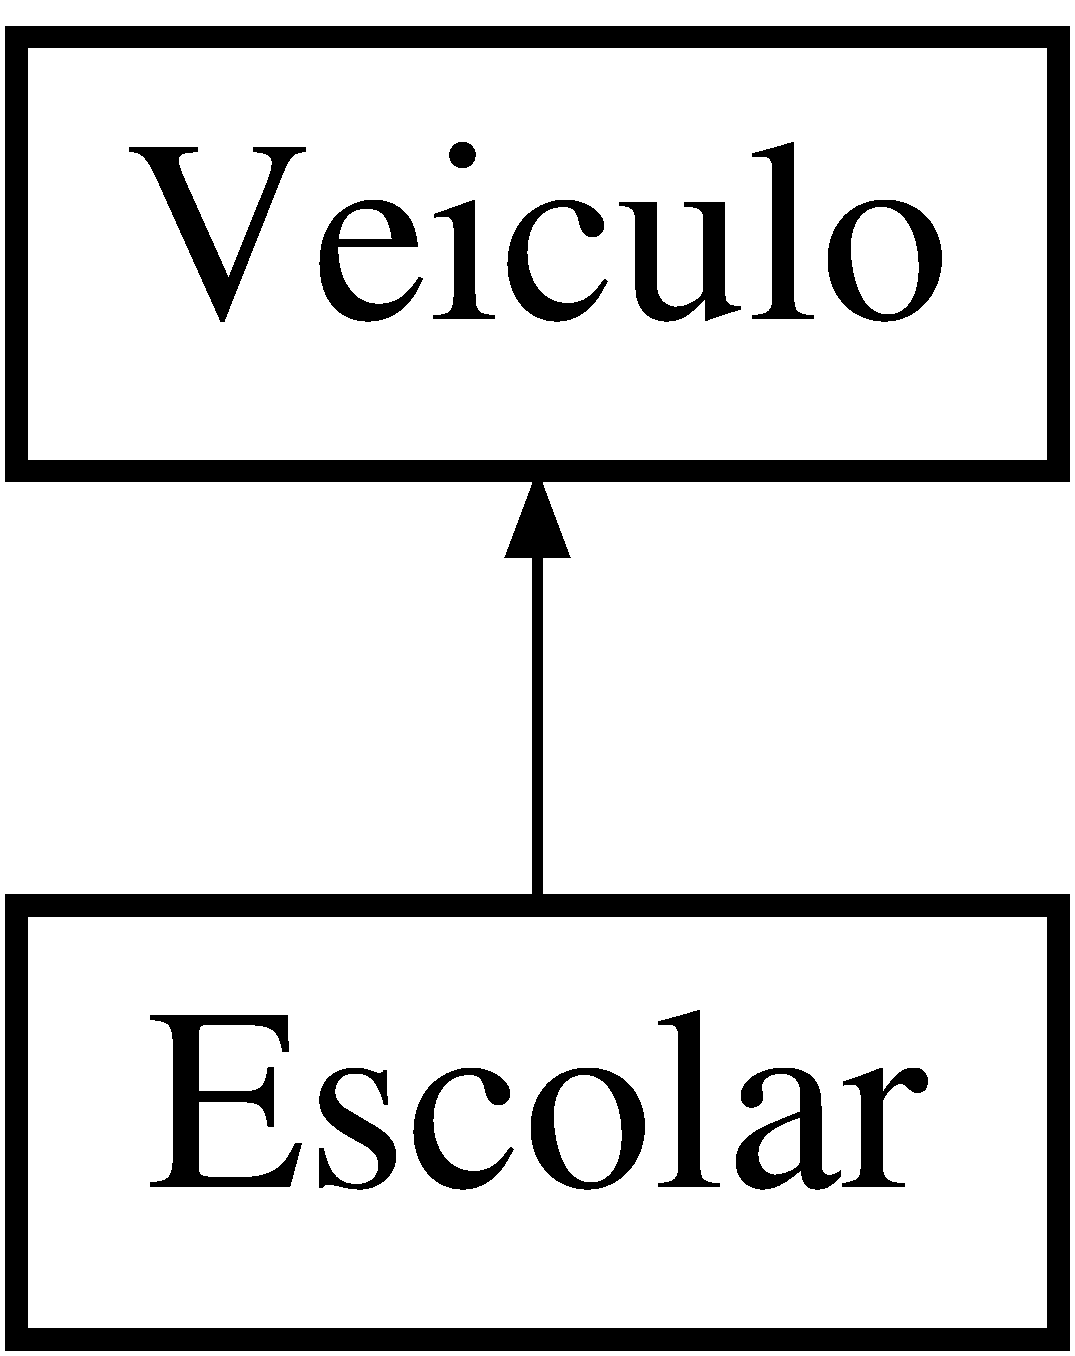
\includegraphics[height=2.000000cm]{class_escolar}
\end{center}
\end{figure}
\subsection*{Public Member Functions}
\begin{DoxyCompactItemize}
\item 
\mbox{\hyperlink{class_escolar_acb87b44d512db57a889d49bfabb25605}{Escolar}} (const string \&\mbox{\hyperlink{class_veiculo_ad9cd698bf39e90508cd0700ee3b9d90b}{matricula}}, float \mbox{\hyperlink{class_veiculo_a06533b15de432c2d6ee86057d35dc547}{consumo100km}}, float \mbox{\hyperlink{class_veiculo_a1b3f7e8c716e8fd68ec7c7405f18c1ef}{preco\+Comb}}, unsigned int capacidade, const vector$<$ unsigned int $>$ \&zonas\+Atravessadas)
\begin{DoxyCompactList}\small\item\em Construtor da classe \mbox{\hyperlink{class_escolar}{Escolar}}. \end{DoxyCompactList}\item 
unsigned int \mbox{\hyperlink{class_escolar_aed580e572a966831deb49bb1736cf7c3}{get\+Lugs\+Livres}} () const
\begin{DoxyCompactList}\small\item\em Permite acesso aos lugares livres no transporte escolar. \end{DoxyCompactList}\item 
vector$<$ unsigned int $>$ \mbox{\hyperlink{class_escolar_a753d9aac081cf11265a1b233531efcbc}{get\+Zonas}} () const
\begin{DoxyCompactList}\small\item\em Permite acesso as zonas atravessadas pelo transporte escolar. \end{DoxyCompactList}\item 
void \mbox{\hyperlink{class_escolar_a8c5ae58b9bf7d7b8ea49097c0a565ebf}{adicionar\+Zona}} (unsigned int zona)
\begin{DoxyCompactList}\small\item\em Adiciona zona ao vetor de zonas atravessadas pelo transporte escolar. \end{DoxyCompactList}\item 
void \mbox{\hyperlink{class_escolar_a17a482658c186318d16d652f34d50c74}{remover\+Zona}} (unsigned int zona)
\begin{DoxyCompactList}\small\item\em Remove a zona do vetor de zonas atravessadas pelo transporte escolar. \end{DoxyCompactList}\item 
bool \mbox{\hyperlink{class_escolar_ae3353410ca33cc4899d2500e24148494}{existe\+Zona}} (unsigned int zona)
\begin{DoxyCompactList}\small\item\em Verifica se o transporte escolar passa pela zona indicada. \end{DoxyCompactList}\item 
float \mbox{\hyperlink{class_escolar_a4834155531d1ba26d0081e59405b14d5}{calc\+Gasto}} (float kms) const
\begin{DoxyCompactList}\small\item\em Calcula o gasto de combustivel do transporte escolar ao fim de um dia. Tendo em conta que realiza duas viagens por dia e o numero de zonas atravessadas, o calculo � 2 $\ast$ numero de zonas atravessadas $\ast$ kms por zona $\ast$ consumo por 100km /100. \end{DoxyCompactList}\item 
bool \mbox{\hyperlink{class_escolar_a9cff84d869113ef8a36dca666f473945}{cheio}} () const
\begin{DoxyCompactList}\small\item\em Verifica se o transporte escolar esta cheio. \end{DoxyCompactList}\item 
\mbox{\Hypertarget{class_escolar_ae8a48df5d876d2d4af02ceab9f3e397c}\label{class_escolar_ae8a48df5d876d2d4af02ceab9f3e397c}} 
void \mbox{\hyperlink{class_escolar_ae8a48df5d876d2d4af02ceab9f3e397c}{aumenta\+Lug}} ()
\begin{DoxyCompactList}\small\item\em Aumenta o numero de lugares vazios em 1. \end{DoxyCompactList}\item 
\mbox{\Hypertarget{class_escolar_a458b5843fe5eba1a8e2d6027487c1ae8}\label{class_escolar_a458b5843fe5eba1a8e2d6027487c1ae8}} 
void \mbox{\hyperlink{class_escolar_a458b5843fe5eba1a8e2d6027487c1ae8}{reduz\+Lug}} ()
\begin{DoxyCompactList}\small\item\em Reduz o numero de lugares vazios em 1. \end{DoxyCompactList}\item 
string \mbox{\hyperlink{class_escolar_aa1f8528c1457656ba5772a253c51b872}{get\+Info}} () const
\begin{DoxyCompactList}\small\item\em Organiza a informacao do transporte escolar para ser guardada em ficheiro. \end{DoxyCompactList}\end{DoxyCompactItemize}
\subsection*{Friends}
\begin{DoxyCompactItemize}
\item 
\mbox{\Hypertarget{class_escolar_aec205505b3b269fb4faece5f16fe94ed}\label{class_escolar_aec205505b3b269fb4faece5f16fe94ed}} 
ostream \& {\bfseries operator$<$$<$} (ostream \&out, const \mbox{\hyperlink{class_escolar}{Escolar}} \&veic)
\end{DoxyCompactItemize}
\subsection*{Additional Inherited Members}


\subsection{Detailed Description}
Classe para instanciar transportes escolares. 

Os transportes escolares sao os responsaveis por levar os utentes de casa ate a escola e vice-\/versa. Por isso cada transporte recreativo possui uma listagem das zonas que atravessa previamente definida para poder levar utentes. 

\subsection{Constructor \& Destructor Documentation}
\mbox{\Hypertarget{class_escolar_acb87b44d512db57a889d49bfabb25605}\label{class_escolar_acb87b44d512db57a889d49bfabb25605}} 
\index{Escolar@{Escolar}!Escolar@{Escolar}}
\index{Escolar@{Escolar}!Escolar@{Escolar}}
\subsubsection{\texorpdfstring{Escolar()}{Escolar()}}
{\footnotesize\ttfamily Escolar\+::\+Escolar (\begin{DoxyParamCaption}\item[{const string \&}]{matricula,  }\item[{float}]{consumo100km,  }\item[{float}]{preco\+Comb,  }\item[{unsigned int}]{capacidade,  }\item[{const vector$<$ unsigned int $>$ \&}]{zonas\+Atravessadas = {\ttfamily vector$<$unsigned~int$>$()} }\end{DoxyParamCaption})}



Construtor da classe \mbox{\hyperlink{class_escolar}{Escolar}}. 


\begin{DoxyParams}{Parameters}
{\em matricula} & Matricula do trasnporte escolar \\
\hline
{\em consumo100km} & Consumo em Litros por cada 100 kms \\
\hline
{\em preco\+Comb} & Preco do combustivel usado no trasnporte escolar \\
\hline
{\em capacidade} & Capacidade total do trasnporte escolar (Inicializa tanto lug\+Totais como lugares\+Livres) \\
\hline
{\em zonas\+Atravessadas} & Vetor das zonas por onde o trasnporte escolar passa (por omissao e inicializado um vector vazio) \\
\hline
\end{DoxyParams}


\subsection{Member Function Documentation}
\mbox{\Hypertarget{class_escolar_a8c5ae58b9bf7d7b8ea49097c0a565ebf}\label{class_escolar_a8c5ae58b9bf7d7b8ea49097c0a565ebf}} 
\index{Escolar@{Escolar}!adicionar\+Zona@{adicionar\+Zona}}
\index{adicionar\+Zona@{adicionar\+Zona}!Escolar@{Escolar}}
\subsubsection{\texorpdfstring{adicionar\+Zona()}{adicionarZona()}}
{\footnotesize\ttfamily void Escolar\+::adicionar\+Zona (\begin{DoxyParamCaption}\item[{unsigned int}]{zona }\end{DoxyParamCaption})\hspace{0.3cm}{\ttfamily [virtual]}}



Adiciona zona ao vetor de zonas atravessadas pelo transporte escolar. 


\begin{DoxyParams}{Parameters}
{\em zona} & Zona a ser adicionada\\
\hline
\end{DoxyParams}
Se a zona ja existir lanca uma excecao do tipo Zona\+Ja\+Existente 

Reimplemented from \mbox{\hyperlink{class_veiculo}{Veiculo}}.

\mbox{\Hypertarget{class_escolar_a4834155531d1ba26d0081e59405b14d5}\label{class_escolar_a4834155531d1ba26d0081e59405b14d5}} 
\index{Escolar@{Escolar}!calc\+Gasto@{calc\+Gasto}}
\index{calc\+Gasto@{calc\+Gasto}!Escolar@{Escolar}}
\subsubsection{\texorpdfstring{calc\+Gasto()}{calcGasto()}}
{\footnotesize\ttfamily float Escolar\+::calc\+Gasto (\begin{DoxyParamCaption}\item[{float}]{kms }\end{DoxyParamCaption}) const\hspace{0.3cm}{\ttfamily [virtual]}}



Calcula o gasto de combustivel do transporte escolar ao fim de um dia. Tendo em conta que realiza duas viagens por dia e o numero de zonas atravessadas, o calculo � 2 $\ast$ numero de zonas atravessadas $\ast$ kms por zona $\ast$ consumo por 100km /100. 


\begin{DoxyParams}{Parameters}
{\em kms} & Media dos kms percorridos por zona atravessada\\
\hline
\end{DoxyParams}
\begin{DoxyReturn}{Returns}
Gasto diario 
\end{DoxyReturn}


Implements \mbox{\hyperlink{class_veiculo}{Veiculo}}.

\mbox{\Hypertarget{class_escolar_a9cff84d869113ef8a36dca666f473945}\label{class_escolar_a9cff84d869113ef8a36dca666f473945}} 
\index{Escolar@{Escolar}!cheio@{cheio}}
\index{cheio@{cheio}!Escolar@{Escolar}}
\subsubsection{\texorpdfstring{cheio()}{cheio()}}
{\footnotesize\ttfamily bool Escolar\+::cheio (\begin{DoxyParamCaption}{ }\end{DoxyParamCaption}) const\hspace{0.3cm}{\ttfamily [virtual]}}



Verifica se o transporte escolar esta cheio. 

\begin{DoxyReturn}{Returns}
true se ja nao houver lugares vazios, false caso contrario 
\end{DoxyReturn}


Reimplemented from \mbox{\hyperlink{class_veiculo}{Veiculo}}.

\mbox{\Hypertarget{class_escolar_ae3353410ca33cc4899d2500e24148494}\label{class_escolar_ae3353410ca33cc4899d2500e24148494}} 
\index{Escolar@{Escolar}!existe\+Zona@{existe\+Zona}}
\index{existe\+Zona@{existe\+Zona}!Escolar@{Escolar}}
\subsubsection{\texorpdfstring{existe\+Zona()}{existeZona()}}
{\footnotesize\ttfamily bool Escolar\+::existe\+Zona (\begin{DoxyParamCaption}\item[{unsigned int}]{zona }\end{DoxyParamCaption})\hspace{0.3cm}{\ttfamily [virtual]}}



Verifica se o transporte escolar passa pela zona indicada. 


\begin{DoxyParams}{Parameters}
{\em zona} & Zona na qual se pretende verificar a passagem\\
\hline
\end{DoxyParams}
\begin{DoxyReturn}{Returns}
true se a zona existe no vetor de zonas atravessadas, false caso contrario 
\end{DoxyReturn}


Reimplemented from \mbox{\hyperlink{class_veiculo}{Veiculo}}.

\mbox{\Hypertarget{class_escolar_aa1f8528c1457656ba5772a253c51b872}\label{class_escolar_aa1f8528c1457656ba5772a253c51b872}} 
\index{Escolar@{Escolar}!get\+Info@{get\+Info}}
\index{get\+Info@{get\+Info}!Escolar@{Escolar}}
\subsubsection{\texorpdfstring{get\+Info()}{getInfo()}}
{\footnotesize\ttfamily string Escolar\+::get\+Info (\begin{DoxyParamCaption}{ }\end{DoxyParamCaption}) const\hspace{0.3cm}{\ttfamily [virtual]}}



Organiza a informacao do transporte escolar para ser guardada em ficheiro. 

\begin{DoxyReturn}{Returns}
string com toda a informacao do transporte escolar (atributos separados por tabs) 
\end{DoxyReturn}


Reimplemented from \mbox{\hyperlink{class_veiculo_a37cf6866bac6b2e7e8837237ec293d48}{Veiculo}}.

\mbox{\Hypertarget{class_escolar_aed580e572a966831deb49bb1736cf7c3}\label{class_escolar_aed580e572a966831deb49bb1736cf7c3}} 
\index{Escolar@{Escolar}!get\+Lugs\+Livres@{get\+Lugs\+Livres}}
\index{get\+Lugs\+Livres@{get\+Lugs\+Livres}!Escolar@{Escolar}}
\subsubsection{\texorpdfstring{get\+Lugs\+Livres()}{getLugsLivres()}}
{\footnotesize\ttfamily unsigned int Escolar\+::get\+Lugs\+Livres (\begin{DoxyParamCaption}{ }\end{DoxyParamCaption}) const\hspace{0.3cm}{\ttfamily [virtual]}}



Permite acesso aos lugares livres no transporte escolar. 

\begin{DoxyReturn}{Returns}
lugares livres no transporte escolar 
\end{DoxyReturn}


Reimplemented from \mbox{\hyperlink{class_veiculo}{Veiculo}}.

\mbox{\Hypertarget{class_escolar_a753d9aac081cf11265a1b233531efcbc}\label{class_escolar_a753d9aac081cf11265a1b233531efcbc}} 
\index{Escolar@{Escolar}!get\+Zonas@{get\+Zonas}}
\index{get\+Zonas@{get\+Zonas}!Escolar@{Escolar}}
\subsubsection{\texorpdfstring{get\+Zonas()}{getZonas()}}
{\footnotesize\ttfamily vector$<$ unsigned int $>$ Escolar\+::get\+Zonas (\begin{DoxyParamCaption}{ }\end{DoxyParamCaption}) const\hspace{0.3cm}{\ttfamily [virtual]}}



Permite acesso as zonas atravessadas pelo transporte escolar. 

\begin{DoxyReturn}{Returns}
vector das zonas atravessadas pelo transporte escolar 
\end{DoxyReturn}


Reimplemented from \mbox{\hyperlink{class_veiculo}{Veiculo}}.

\mbox{\Hypertarget{class_escolar_a17a482658c186318d16d652f34d50c74}\label{class_escolar_a17a482658c186318d16d652f34d50c74}} 
\index{Escolar@{Escolar}!remover\+Zona@{remover\+Zona}}
\index{remover\+Zona@{remover\+Zona}!Escolar@{Escolar}}
\subsubsection{\texorpdfstring{remover\+Zona()}{removerZona()}}
{\footnotesize\ttfamily void Escolar\+::remover\+Zona (\begin{DoxyParamCaption}\item[{unsigned int}]{zona }\end{DoxyParamCaption})\hspace{0.3cm}{\ttfamily [virtual]}}



Remove a zona do vetor de zonas atravessadas pelo transporte escolar. 


\begin{DoxyParams}{Parameters}
{\em zona} & Zona a ser removida\\
\hline
\end{DoxyParams}
Se a zona nao existir lanca uma excecao do tipo Zona\+Nao\+Existente 

Reimplemented from \mbox{\hyperlink{class_veiculo}{Veiculo}}.



The documentation for this class was generated from the following files\+:\begin{DoxyCompactItemize}
\item 
C\+:/\+Users/\+Cajo/\+Desktop/\+Repos/\+A\+E\+D\+A-\/\+P\+R\+O\+J1/src/Veiculo.\+h\item 
C\+:/\+Users/\+Cajo/\+Desktop/\+Repos/\+A\+E\+D\+A-\/\+P\+R\+O\+J1/src/Veiculo.\+cpp\end{DoxyCompactItemize}

\hypertarget{class_funcionario}{}\section{Funcionario Class Reference}
\label{class_funcionario}\index{Funcionario@{Funcionario}}


Classe para instanciar funcionarios.  




{\ttfamily \#include $<$Utente.\+h$>$}

Inheritance diagram for Funcionario\+:\begin{figure}[H]
\begin{center}
\leavevmode
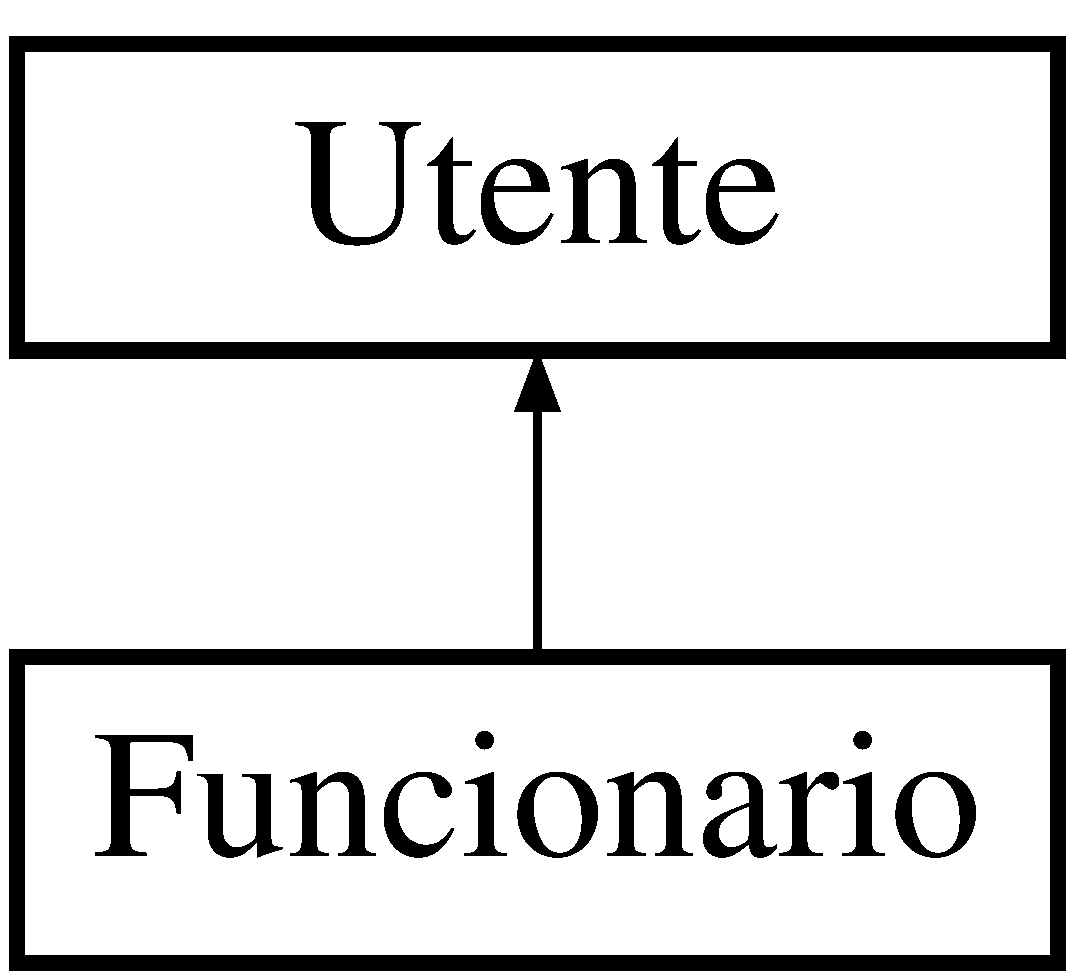
\includegraphics[height=2.000000cm]{class_funcionario}
\end{center}
\end{figure}
\subsection*{Public Member Functions}
\begin{DoxyCompactItemize}
\item 
\mbox{\hyperlink{class_funcionario_ac6e6169c18146e5fd2c67e6ccd0ebe75}{Funcionario}} (const string \&\mbox{\hyperlink{class_utente_a328c722d27759eaa88596ccb4cf2549f}{nome}}, const string \&data\+\_\+nasc, const string \&\mbox{\hyperlink{class_utente_ac5acf8e42ccd10808d077fc0db2e05f9}{BI}}, const unsigned int \&zona\+Habit, const unsigned int \&zona\+Esc, const bool \&docente, const unsigned int \&contacto)
\begin{DoxyCompactList}\small\item\em Construtor da classe \mbox{\hyperlink{class_funcionario}{Funcionario}}. \end{DoxyCompactList}\item 
bool \mbox{\hyperlink{class_funcionario_a298a2b333cae15e6f426890c2a352dc2}{get\+Docente}} ()
\begin{DoxyCompactList}\small\item\em Permite acesso ao estatuto do funcionario na escola. \end{DoxyCompactList}\item 
unsigned int \mbox{\hyperlink{class_funcionario_a408d2f4ac6ebdebbc18072832fce9ef7}{get\+Contacto}} () const
\begin{DoxyCompactList}\small\item\em Permite acesso ao contacto do funcionario. \end{DoxyCompactList}\item 
void \mbox{\hyperlink{class_funcionario_a2288d370e92da8b533c09db5b90d888c}{set\+Contacto}} (unsigned int cont)
\begin{DoxyCompactList}\small\item\em Altera o contacto do funcionario. \end{DoxyCompactList}\item 
string \mbox{\hyperlink{class_funcionario_a3cafb55c689dcb260975d3083cef1a98}{get\+Info}} () const
\begin{DoxyCompactList}\small\item\em Organiza a informacao do funcionario para ser guardada em ficheiro. \end{DoxyCompactList}\end{DoxyCompactItemize}
\subsection*{Friends}
\begin{DoxyCompactItemize}
\item 
\mbox{\Hypertarget{class_funcionario_adea2bb01573fbd53fea2ebaa08f82e92}\label{class_funcionario_adea2bb01573fbd53fea2ebaa08f82e92}} 
ostream \& {\bfseries operator$<$$<$} (ostream \&out, const \mbox{\hyperlink{class_funcionario}{Funcionario}} \&utente)
\end{DoxyCompactItemize}
\subsection*{Additional Inherited Members}


\subsection{Detailed Description}
Classe para instanciar funcionarios. 

Para alem das caracteristicas de um utente normal, o funcionario pode ou nao ser docente e tem um numero de telemovel associado. 

\subsection{Constructor \& Destructor Documentation}
\mbox{\Hypertarget{class_funcionario_ac6e6169c18146e5fd2c67e6ccd0ebe75}\label{class_funcionario_ac6e6169c18146e5fd2c67e6ccd0ebe75}} 
\index{Funcionario@{Funcionario}!Funcionario@{Funcionario}}
\index{Funcionario@{Funcionario}!Funcionario@{Funcionario}}
\subsubsection{\texorpdfstring{Funcionario()}{Funcionario()}}
{\footnotesize\ttfamily Funcionario\+::\+Funcionario (\begin{DoxyParamCaption}\item[{const string \&}]{nome,  }\item[{const string \&}]{data\+\_\+nasc,  }\item[{const string \&}]{BI,  }\item[{const unsigned int \&}]{zona\+Habit,  }\item[{const unsigned int \&}]{zona\+Esc,  }\item[{const bool \&}]{docente,  }\item[{const unsigned int \&}]{contacto }\end{DoxyParamCaption})}



Construtor da classe \mbox{\hyperlink{class_funcionario}{Funcionario}}. 


\begin{DoxyParams}{Parameters}
{\em nome} & Nome do funcionario \\
\hline
{\em data\+\_\+nasc} & Data de nascimento \\
\hline
{\em BI} & BI do funcionario \\
\hline
{\em zona\+Habit} & Zona de habitacao do funcionario \\
\hline
{\em zona\+Esc} & Zona da escola do funcionario \\
\hline
{\em docente} & True se o funcionario � docente, False caso contrario \\
\hline
{\em contacto} & Contacto do funcionario \\
\hline
\end{DoxyParams}


\subsection{Member Function Documentation}
\mbox{\Hypertarget{class_funcionario_a408d2f4ac6ebdebbc18072832fce9ef7}\label{class_funcionario_a408d2f4ac6ebdebbc18072832fce9ef7}} 
\index{Funcionario@{Funcionario}!get\+Contacto@{get\+Contacto}}
\index{get\+Contacto@{get\+Contacto}!Funcionario@{Funcionario}}
\subsubsection{\texorpdfstring{get\+Contacto()}{getContacto()}}
{\footnotesize\ttfamily unsigned int Funcionario\+::get\+Contacto (\begin{DoxyParamCaption}{ }\end{DoxyParamCaption}) const\hspace{0.3cm}{\ttfamily [virtual]}}



Permite acesso ao contacto do funcionario. 

\begin{DoxyReturn}{Returns}
contacto do funcionario (unsigned int) 
\end{DoxyReturn}


Implements \mbox{\hyperlink{class_utente}{Utente}}.

\mbox{\Hypertarget{class_funcionario_a298a2b333cae15e6f426890c2a352dc2}\label{class_funcionario_a298a2b333cae15e6f426890c2a352dc2}} 
\index{Funcionario@{Funcionario}!get\+Docente@{get\+Docente}}
\index{get\+Docente@{get\+Docente}!Funcionario@{Funcionario}}
\subsubsection{\texorpdfstring{get\+Docente()}{getDocente()}}
{\footnotesize\ttfamily bool Funcionario\+::get\+Docente (\begin{DoxyParamCaption}{ }\end{DoxyParamCaption})\hspace{0.3cm}{\ttfamily [virtual]}}



Permite acesso ao estatuto do funcionario na escola. 

\begin{DoxyReturn}{Returns}
true se o funcionario for docente, falso caso contrario 
\end{DoxyReturn}


Reimplemented from \mbox{\hyperlink{class_utente}{Utente}}.

\mbox{\Hypertarget{class_funcionario_a3cafb55c689dcb260975d3083cef1a98}\label{class_funcionario_a3cafb55c689dcb260975d3083cef1a98}} 
\index{Funcionario@{Funcionario}!get\+Info@{get\+Info}}
\index{get\+Info@{get\+Info}!Funcionario@{Funcionario}}
\subsubsection{\texorpdfstring{get\+Info()}{getInfo()}}
{\footnotesize\ttfamily string Funcionario\+::get\+Info (\begin{DoxyParamCaption}{ }\end{DoxyParamCaption}) const\hspace{0.3cm}{\ttfamily [virtual]}}



Organiza a informacao do funcionario para ser guardada em ficheiro. 

\begin{DoxyReturn}{Returns}
string com toda a informacao do funcionario (atributos separados por tabs) 
\end{DoxyReturn}


Reimplemented from \mbox{\hyperlink{class_utente_aee03eae2a7154e7b4713b2be195d548f}{Utente}}.

\mbox{\Hypertarget{class_funcionario_a2288d370e92da8b533c09db5b90d888c}\label{class_funcionario_a2288d370e92da8b533c09db5b90d888c}} 
\index{Funcionario@{Funcionario}!set\+Contacto@{set\+Contacto}}
\index{set\+Contacto@{set\+Contacto}!Funcionario@{Funcionario}}
\subsubsection{\texorpdfstring{set\+Contacto()}{setContacto()}}
{\footnotesize\ttfamily void Funcionario\+::set\+Contacto (\begin{DoxyParamCaption}\item[{unsigned int}]{cont }\end{DoxyParamCaption})\hspace{0.3cm}{\ttfamily [virtual]}}



Altera o contacto do funcionario. 


\begin{DoxyParams}{Parameters}
{\em cont} & Novo contacto do funcionario \\
\hline
\end{DoxyParams}


Implements \mbox{\hyperlink{class_utente}{Utente}}.



The documentation for this class was generated from the following files\+:\begin{DoxyCompactItemize}
\item 
C\+:/\+Users/\+Cajo/\+Desktop/\+Repos/\+A\+E\+D\+A-\/\+P\+R\+O\+J1/src/Utente.\+h\item 
C\+:/\+Users/\+Cajo/\+Desktop/\+Repos/\+A\+E\+D\+A-\/\+P\+R\+O\+J1/src/Utente.\+cpp\end{DoxyCompactItemize}

\hypertarget{class_recreativo}{}\section{Recreativo Class Reference}
\label{class_recreativo}\index{Recreativo@{Recreativo}}


Classe para instanciar transportes de atividades recreativas.  




{\ttfamily \#include $<$Veiculo.\+h$>$}

Inheritance diagram for Recreativo\+:\begin{figure}[H]
\begin{center}
\leavevmode
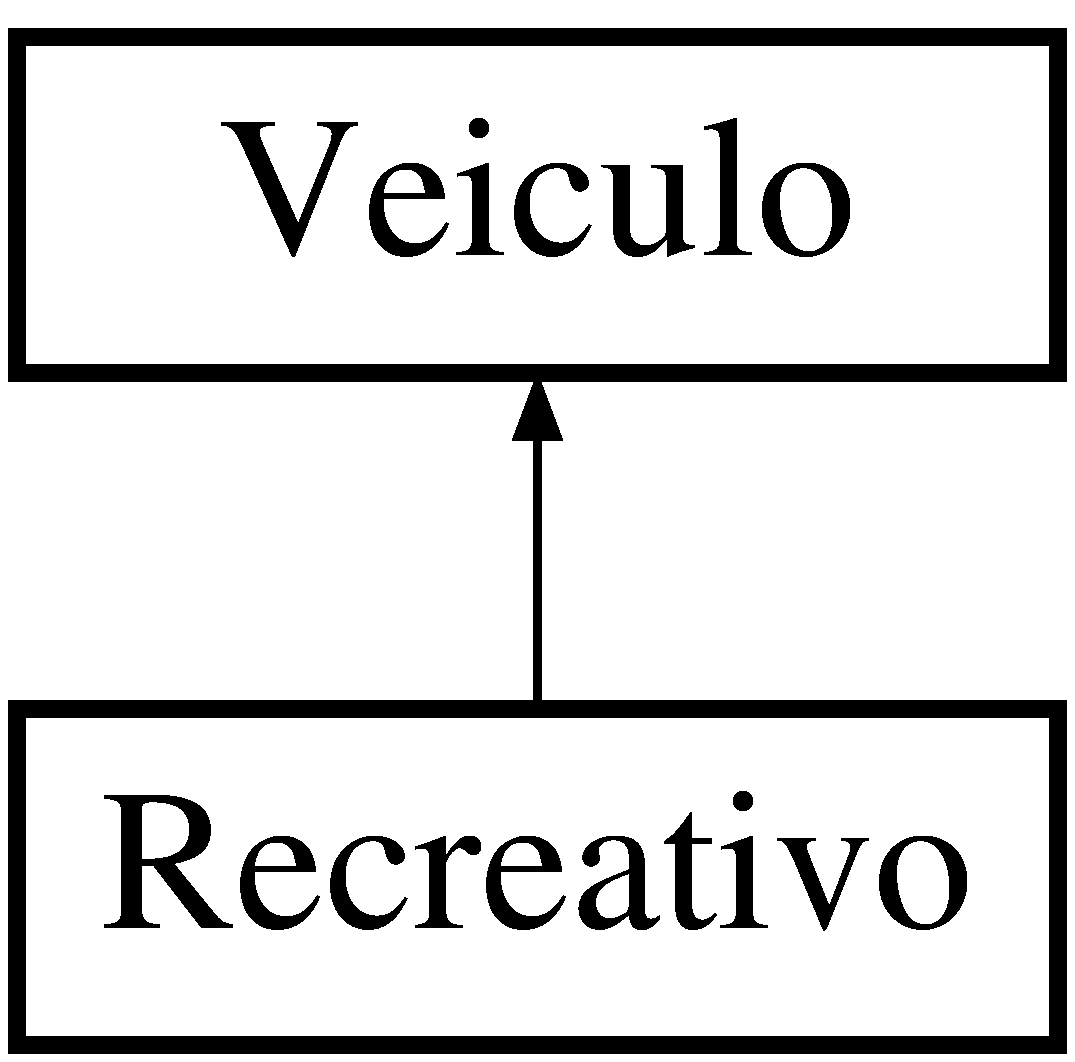
\includegraphics[height=2.000000cm]{class_recreativo}
\end{center}
\end{figure}
\subsection*{Public Member Functions}
\begin{DoxyCompactItemize}
\item 
\mbox{\hyperlink{class_recreativo_aa931f6746a37e943b28387afed12ba34}{Recreativo}} (const string \&\mbox{\hyperlink{class_veiculo_ad9cd698bf39e90508cd0700ee3b9d90b}{matricula}}, float \mbox{\hyperlink{class_veiculo_a06533b15de432c2d6ee86057d35dc547}{consumo100km}}, float \mbox{\hyperlink{class_veiculo_a1b3f7e8c716e8fd68ec7c7405f18c1ef}{preco\+Comb}}, unsigned int cap, bool alugado)
\begin{DoxyCompactList}\small\item\em Construtor da classe \mbox{\hyperlink{class_recreativo}{Recreativo}}. \end{DoxyCompactList}\item 
unsigned int \mbox{\hyperlink{class_recreativo_ac03c531c9508b88ba3ebae98a906063e}{get\+Capacidade}} () const
\begin{DoxyCompactList}\small\item\em Permite acesso a capacidade do transporte recreativo. \end{DoxyCompactList}\item 
bool \mbox{\hyperlink{class_recreativo_a53798a5ad2a1b230927f29e6aa155272}{get\+Estado}} () const
\begin{DoxyCompactList}\small\item\em Permite acesso ao estado de aluguer do transporte recreativo. \end{DoxyCompactList}\item 
void \mbox{\hyperlink{class_recreativo_a43fca1861ff7f7f068fe303cb8f44d3d}{set\+Estado}} (bool alugado)
\begin{DoxyCompactList}\small\item\em Altera o estado de aluguer do veiculo recreativo. \end{DoxyCompactList}\item 
float \mbox{\hyperlink{class_recreativo_a83557bafb258efa9686ea2c2beb05442}{calc\+Gasto}} (float kms) const
\begin{DoxyCompactList}\small\item\em Calcula o gasto de combustivel do transporte recreativo ao fim de uma viagem. O gasto depende dos kms percorridos na viagem e do consumo por 100km do veiculo. \end{DoxyCompactList}\item 
string \mbox{\hyperlink{class_recreativo_a594c854bbcb834cff82c0687afa2b9ce}{get\+Info}} () const
\begin{DoxyCompactList}\small\item\em Organiza a informacao do transporte recreativo para ser guardada em ficheiro. \end{DoxyCompactList}\end{DoxyCompactItemize}
\subsection*{Friends}
\begin{DoxyCompactItemize}
\item 
\mbox{\Hypertarget{class_recreativo_a207796b1dc2e32b04fb075791f87e193}\label{class_recreativo_a207796b1dc2e32b04fb075791f87e193}} 
ostream \& {\bfseries operator$<$$<$} (ostream \&out, const \mbox{\hyperlink{class_recreativo}{Recreativo}} \&veic)
\end{DoxyCompactItemize}
\subsection*{Additional Inherited Members}


\subsection{Detailed Description}
Classe para instanciar transportes de atividades recreativas. 

Veiculos especiais que se podem alugar por um dia. O preco do aluguer depende da capacidade do transporte recreativo (atributo constante). Caso ele tenha sido alugado para o dia, e tambem importante calcular o gasto correspondente. 

\subsection{Constructor \& Destructor Documentation}
\mbox{\Hypertarget{class_recreativo_aa931f6746a37e943b28387afed12ba34}\label{class_recreativo_aa931f6746a37e943b28387afed12ba34}} 
\index{Recreativo@{Recreativo}!Recreativo@{Recreativo}}
\index{Recreativo@{Recreativo}!Recreativo@{Recreativo}}
\subsubsection{\texorpdfstring{Recreativo()}{Recreativo()}}
{\footnotesize\ttfamily Recreativo\+::\+Recreativo (\begin{DoxyParamCaption}\item[{const string \&}]{matricula,  }\item[{float}]{consumo100km,  }\item[{float}]{preco\+Comb,  }\item[{unsigned int}]{cap,  }\item[{bool}]{alugado = {\ttfamily false} }\end{DoxyParamCaption})}



Construtor da classe \mbox{\hyperlink{class_recreativo}{Recreativo}}. 


\begin{DoxyParams}{Parameters}
{\em matricula} & Matricula do trasnporte recreativo \\
\hline
{\em consumo100km} & Consumo em Litros por cada 100 kms \\
\hline
{\em preco\+Comb} & Preco do combustivel usado no trasnporte recreativo \\
\hline
{\em cap} & Capacidade do trasnporte recreativo \\
\hline
{\em alugado} & Estado de aluguer do transporte recreativo (true-\/$>$alugado, false-\/$>$livre). Por omissao e false. \\
\hline
\end{DoxyParams}


\subsection{Member Function Documentation}
\mbox{\Hypertarget{class_recreativo_a83557bafb258efa9686ea2c2beb05442}\label{class_recreativo_a83557bafb258efa9686ea2c2beb05442}} 
\index{Recreativo@{Recreativo}!calc\+Gasto@{calc\+Gasto}}
\index{calc\+Gasto@{calc\+Gasto}!Recreativo@{Recreativo}}
\subsubsection{\texorpdfstring{calc\+Gasto()}{calcGasto()}}
{\footnotesize\ttfamily float Recreativo\+::calc\+Gasto (\begin{DoxyParamCaption}\item[{float}]{kms }\end{DoxyParamCaption}) const\hspace{0.3cm}{\ttfamily [virtual]}}



Calcula o gasto de combustivel do transporte recreativo ao fim de uma viagem. O gasto depende dos kms percorridos na viagem e do consumo por 100km do veiculo. 


\begin{DoxyParams}{Parameters}
{\em kms} & Kms percorridos durante a viagem\\
\hline
\end{DoxyParams}
\begin{DoxyReturn}{Returns}
Gasto na viagem 
\end{DoxyReturn}


Implements \mbox{\hyperlink{class_veiculo}{Veiculo}}.

\mbox{\Hypertarget{class_recreativo_ac03c531c9508b88ba3ebae98a906063e}\label{class_recreativo_ac03c531c9508b88ba3ebae98a906063e}} 
\index{Recreativo@{Recreativo}!get\+Capacidade@{get\+Capacidade}}
\index{get\+Capacidade@{get\+Capacidade}!Recreativo@{Recreativo}}
\subsubsection{\texorpdfstring{get\+Capacidade()}{getCapacidade()}}
{\footnotesize\ttfamily unsigned int Recreativo\+::get\+Capacidade (\begin{DoxyParamCaption}{ }\end{DoxyParamCaption}) const\hspace{0.3cm}{\ttfamily [virtual]}}



Permite acesso a capacidade do transporte recreativo. 

\begin{DoxyReturn}{Returns}
capacidade do transporte recreativo 
\end{DoxyReturn}


Reimplemented from \mbox{\hyperlink{class_veiculo}{Veiculo}}.

\mbox{\Hypertarget{class_recreativo_a53798a5ad2a1b230927f29e6aa155272}\label{class_recreativo_a53798a5ad2a1b230927f29e6aa155272}} 
\index{Recreativo@{Recreativo}!get\+Estado@{get\+Estado}}
\index{get\+Estado@{get\+Estado}!Recreativo@{Recreativo}}
\subsubsection{\texorpdfstring{get\+Estado()}{getEstado()}}
{\footnotesize\ttfamily bool Recreativo\+::get\+Estado (\begin{DoxyParamCaption}{ }\end{DoxyParamCaption}) const\hspace{0.3cm}{\ttfamily [virtual]}}



Permite acesso ao estado de aluguer do transporte recreativo. 

\begin{DoxyReturn}{Returns}
true se o transporte recreativo estiver alugado, false caso contrario 
\end{DoxyReturn}


Reimplemented from \mbox{\hyperlink{class_veiculo}{Veiculo}}.

\mbox{\Hypertarget{class_recreativo_a594c854bbcb834cff82c0687afa2b9ce}\label{class_recreativo_a594c854bbcb834cff82c0687afa2b9ce}} 
\index{Recreativo@{Recreativo}!get\+Info@{get\+Info}}
\index{get\+Info@{get\+Info}!Recreativo@{Recreativo}}
\subsubsection{\texorpdfstring{get\+Info()}{getInfo()}}
{\footnotesize\ttfamily string Recreativo\+::get\+Info (\begin{DoxyParamCaption}{ }\end{DoxyParamCaption}) const\hspace{0.3cm}{\ttfamily [virtual]}}



Organiza a informacao do transporte recreativo para ser guardada em ficheiro. 

\begin{DoxyReturn}{Returns}
string com toda a informacao do transporte recreativo (atributos separados por tabs) 
\end{DoxyReturn}


Reimplemented from \mbox{\hyperlink{class_veiculo_a37cf6866bac6b2e7e8837237ec293d48}{Veiculo}}.

\mbox{\Hypertarget{class_recreativo_a43fca1861ff7f7f068fe303cb8f44d3d}\label{class_recreativo_a43fca1861ff7f7f068fe303cb8f44d3d}} 
\index{Recreativo@{Recreativo}!set\+Estado@{set\+Estado}}
\index{set\+Estado@{set\+Estado}!Recreativo@{Recreativo}}
\subsubsection{\texorpdfstring{set\+Estado()}{setEstado()}}
{\footnotesize\ttfamily void Recreativo\+::set\+Estado (\begin{DoxyParamCaption}\item[{bool}]{alugado }\end{DoxyParamCaption})\hspace{0.3cm}{\ttfamily [virtual]}}



Altera o estado de aluguer do veiculo recreativo. 


\begin{DoxyParams}{Parameters}
{\em alugado} & Estado de aluguer do veiculo (true-\/$>$alugado, false-\/$>$livre) \\
\hline
\end{DoxyParams}


Reimplemented from \mbox{\hyperlink{class_veiculo}{Veiculo}}.



The documentation for this class was generated from the following files\+:\begin{DoxyCompactItemize}
\item 
C\+:/\+Users/\+Cajo/\+Desktop/\+Repos/\+A\+E\+D\+A-\/\+P\+R\+O\+J1/src/Veiculo.\+h\item 
C\+:/\+Users/\+Cajo/\+Desktop/\+Repos/\+A\+E\+D\+A-\/\+P\+R\+O\+J1/src/Veiculo.\+cpp\end{DoxyCompactItemize}

\hypertarget{class_utente}{}\section{Utente Class Reference}
\label{class_utente}\index{Utente@{Utente}}


Classe para instanciar utentes.  




{\ttfamily \#include $<$Utente.\+h$>$}

Inheritance diagram for Utente\+:\begin{figure}[H]
\begin{center}
\leavevmode
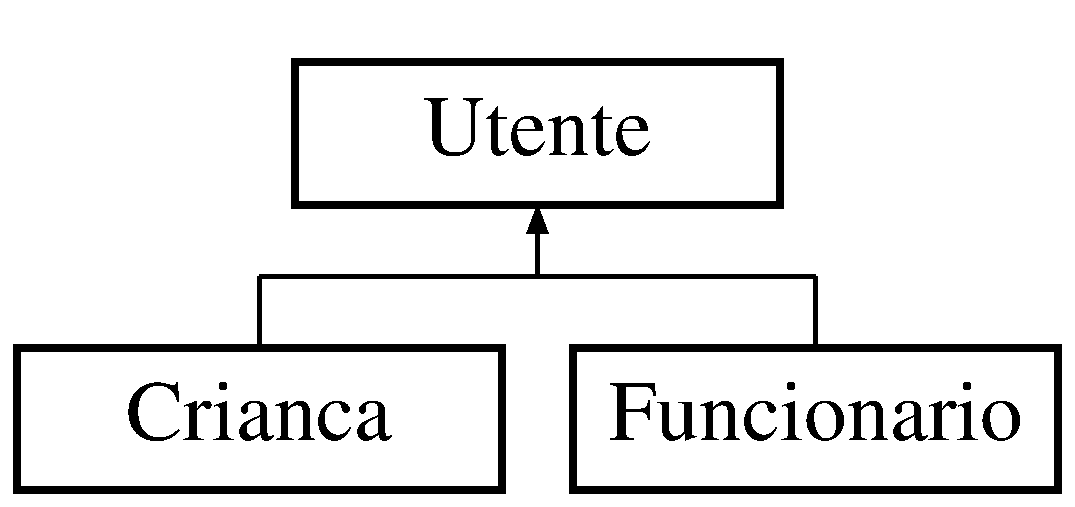
\includegraphics[height=2.000000cm]{class_utente}
\end{center}
\end{figure}
\subsection*{Public Member Functions}
\begin{DoxyCompactItemize}
\item 
\mbox{\hyperlink{class_utente_adf216e1f6792b96c6404aae73121d44d}{Utente}} (const string \&\mbox{\hyperlink{class_utente_a328c722d27759eaa88596ccb4cf2549f}{nome}}, const string \&data\+\_\+nasc, const string \&\mbox{\hyperlink{class_utente_ac5acf8e42ccd10808d077fc0db2e05f9}{BI}}, const unsigned int \&zona\+Habit, const unsigned int \&zona\+Esc)
\begin{DoxyCompactList}\small\item\em Construtor da classe \mbox{\hyperlink{class_utente}{Utente}}. \end{DoxyCompactList}\item 
string \mbox{\hyperlink{class_utente_a56bf08dbd5fb7fd208421cae1105d9e4}{get\+Nome}} ()
\begin{DoxyCompactList}\small\item\em Permite acesso ao nome do utente. \end{DoxyCompactList}\item 
string \mbox{\hyperlink{class_utente_a71bbb2b8ae7bc703c983601653b8bd0e}{get\+Data\+\_\+\+Nasc}} ()
\begin{DoxyCompactList}\small\item\em Permite acesso a data de nascimento do utente. \end{DoxyCompactList}\item 
string \mbox{\hyperlink{class_utente_a4f00a92ad23d9b42e799e90444f0b99f}{get\+BI}} ()
\begin{DoxyCompactList}\small\item\em Permite acesso ao BI do utente. \end{DoxyCompactList}\item 
unsigned int \mbox{\hyperlink{class_utente_a02e1b87d26c3770a70e01ecdc7cf87f2}{get\+Num\+Utente}} ()
\begin{DoxyCompactList}\small\item\em Devolve o numero de identificacao interna do utente. \end{DoxyCompactList}\item 
unsigned int \mbox{\hyperlink{class_utente_a69163220b163eeef2359745f9d7b92c2}{get\+Zona\+Habitacao}} ()
\begin{DoxyCompactList}\small\item\em Devolve a zona onde o utente habita. \end{DoxyCompactList}\item 
unsigned int \mbox{\hyperlink{class_utente_a9f7ee5806d6a187cf8ab27c2bd36c501}{get\+Zona\+Escola}} ()
\begin{DoxyCompactList}\small\item\em Devolve a zona da escola do utente. \end{DoxyCompactList}\item 
void \mbox{\hyperlink{class_utente_a7276cad0368359751b7aad74ed305806}{set\+Zona\+Habitacao}} (unsigned int zona)
\begin{DoxyCompactList}\small\item\em Altera a zona de habitacao do utente. \end{DoxyCompactList}\item 
void \mbox{\hyperlink{class_utente_ad6d072f72c3d373bbb0a7ace551fff55}{set\+Zona\+Escola}} (unsigned int zona)
\begin{DoxyCompactList}\small\item\em Altera a zona da escola do utente. \end{DoxyCompactList}\item 
\mbox{\Hypertarget{class_utente_a899016287b536c9b1feaf8d442b67c5b}\label{class_utente_a899016287b536c9b1feaf8d442b67c5b}} 
virtual unsigned int {\bfseries get\+Contacto} () const =0
\item 
\mbox{\Hypertarget{class_utente_a0c9a0884b16349201f12fd75dd6c4184}\label{class_utente_a0c9a0884b16349201f12fd75dd6c4184}} 
virtual void {\bfseries set\+Contacto} (unsigned int cont)=0
\item 
\mbox{\Hypertarget{class_utente_a6633751f30f241cbb95152f09d69c413}\label{class_utente_a6633751f30f241cbb95152f09d69c413}} 
virtual string {\bfseries get\+Nome\+EE} () const
\item 
\mbox{\Hypertarget{class_utente_a004a0a657b7f44cfe19e94c336d1ad6b}\label{class_utente_a004a0a657b7f44cfe19e94c336d1ad6b}} 
virtual bool {\bfseries get\+Docente} ()
\item 
virtual string \mbox{\hyperlink{class_utente_aee03eae2a7154e7b4713b2be195d548f}{get\+Info}} () const
\begin{DoxyCompactList}\small\item\em Organiza a informacao do utente para ser guardada em ficheiro. \end{DoxyCompactList}\end{DoxyCompactItemize}
\subsection*{Static Public Attributes}
\begin{DoxyCompactItemize}
\item 
\mbox{\Hypertarget{class_utente_a61402075e3df7b7b21e141ea7e1b5f0f}\label{class_utente_a61402075e3df7b7b21e141ea7e1b5f0f}} 
static unsigned int \mbox{\hyperlink{class_utente_a61402075e3df7b7b21e141ea7e1b5f0f}{ult\+\_\+num\+Utente}} = 0
\begin{DoxyCompactList}\small\item\em Membro estatico que guarda qual o numero de identificacao do ultimo utente registado. \end{DoxyCompactList}\end{DoxyCompactItemize}
\subsection*{Protected Attributes}
\begin{DoxyCompactItemize}
\item 
\mbox{\Hypertarget{class_utente_a328c722d27759eaa88596ccb4cf2549f}\label{class_utente_a328c722d27759eaa88596ccb4cf2549f}} 
const string \mbox{\hyperlink{class_utente_a328c722d27759eaa88596ccb4cf2549f}{nome}}
\begin{DoxyCompactList}\small\item\em Nome do utente. \end{DoxyCompactList}\item 
\mbox{\Hypertarget{class_utente_a04d2aeac0b14725caa1066a1c34806f1}\label{class_utente_a04d2aeac0b14725caa1066a1c34806f1}} 
const string \mbox{\hyperlink{class_utente_a04d2aeac0b14725caa1066a1c34806f1}{data\+\_\+nascimento}}
\begin{DoxyCompactList}\small\item\em Data de nascimento do utente (Nota\+: nao e controlado o input) \end{DoxyCompactList}\item 
\mbox{\Hypertarget{class_utente_ac5acf8e42ccd10808d077fc0db2e05f9}\label{class_utente_ac5acf8e42ccd10808d077fc0db2e05f9}} 
const string \mbox{\hyperlink{class_utente_ac5acf8e42ccd10808d077fc0db2e05f9}{BI}}
\begin{DoxyCompactList}\small\item\em BI do utente (Nota\+: nao ha BI\textquotesingle{}s repetidos) \end{DoxyCompactList}\item 
\mbox{\Hypertarget{class_utente_ac1bde470c6fa7d57665c6d7fa24c90f2}\label{class_utente_ac1bde470c6fa7d57665c6d7fa24c90f2}} 
unsigned int \mbox{\hyperlink{class_utente_ac1bde470c6fa7d57665c6d7fa24c90f2}{num\+Utente}}
\begin{DoxyCompactList}\small\item\em Numero de identificacao interna do utente. \end{DoxyCompactList}\item 
\mbox{\Hypertarget{class_utente_a424e352516988e1ad851c7433a512463}\label{class_utente_a424e352516988e1ad851c7433a512463}} 
unsigned int \mbox{\hyperlink{class_utente_a424e352516988e1ad851c7433a512463}{zona\+Habitacao}}
\begin{DoxyCompactList}\small\item\em Zona onde o utente habita. \end{DoxyCompactList}\item 
\mbox{\Hypertarget{class_utente_a435d662e6cfc7f767e3d7afbba97a530}\label{class_utente_a435d662e6cfc7f767e3d7afbba97a530}} 
unsigned int \mbox{\hyperlink{class_utente_a435d662e6cfc7f767e3d7afbba97a530}{zona\+Escola}}
\begin{DoxyCompactList}\small\item\em Zona da escola do utente. \end{DoxyCompactList}\end{DoxyCompactItemize}
\subsection*{Friends}
\begin{DoxyCompactItemize}
\item 
\mbox{\Hypertarget{class_utente_ad9960100ba421bb4e54879250b47dcdf}\label{class_utente_ad9960100ba421bb4e54879250b47dcdf}} 
ostream \& {\bfseries operator$<$$<$} (ostream \&out, const \mbox{\hyperlink{class_utente}{Utente}} \&utente)
\end{DoxyCompactItemize}


\subsection{Detailed Description}
Classe para instanciar utentes. 

Esta classe agrupa todas as caracteristicas de um utente. Permite definir os clientes da empresa de transportes e operar sobre alguns dos aspectos mais importantes, como por exemplo\+: verificar quais as zonas onde o cliente habita e tem escola, verificar se um cliente e utente ou funcionario, encontrar o numero de telemovel do cliente para o poder contactar, etc. Da classe \mbox{\hyperlink{class_utente}{Utente}} derivam a classe \mbox{\hyperlink{class_crianca}{Crianca}} e a classe \mbox{\hyperlink{class_funcionario}{Funcionario}}. 

\subsection{Constructor \& Destructor Documentation}
\mbox{\Hypertarget{class_utente_adf216e1f6792b96c6404aae73121d44d}\label{class_utente_adf216e1f6792b96c6404aae73121d44d}} 
\index{Utente@{Utente}!Utente@{Utente}}
\index{Utente@{Utente}!Utente@{Utente}}
\subsubsection{\texorpdfstring{Utente()}{Utente()}}
{\footnotesize\ttfamily Utente\+::\+Utente (\begin{DoxyParamCaption}\item[{const string \&}]{nome,  }\item[{const string \&}]{data\+\_\+nasc,  }\item[{const string \&}]{BI,  }\item[{const unsigned int \&}]{zona\+Habit,  }\item[{const unsigned int \&}]{zona\+Esc }\end{DoxyParamCaption})}



Construtor da classe \mbox{\hyperlink{class_utente}{Utente}}. 


\begin{DoxyParams}{Parameters}
{\em nome} & Nome do utente \\
\hline
{\em data\+\_\+nasc} & Data de nascimento \\
\hline
{\em BI} & BI do utente \\
\hline
{\em zona\+Habit} & Zona de habitacao do utente \\
\hline
{\em zona\+Esc} & Zona da escola do utente \\
\hline
\end{DoxyParams}


\subsection{Member Function Documentation}
\mbox{\Hypertarget{class_utente_a4f00a92ad23d9b42e799e90444f0b99f}\label{class_utente_a4f00a92ad23d9b42e799e90444f0b99f}} 
\index{Utente@{Utente}!get\+BI@{get\+BI}}
\index{get\+BI@{get\+BI}!Utente@{Utente}}
\subsubsection{\texorpdfstring{get\+B\+I()}{getBI()}}
{\footnotesize\ttfamily string Utente\+::get\+BI (\begin{DoxyParamCaption}{ }\end{DoxyParamCaption})}



Permite acesso ao BI do utente. 

\begin{DoxyReturn}{Returns}
BI do utente 
\end{DoxyReturn}
\mbox{\Hypertarget{class_utente_a71bbb2b8ae7bc703c983601653b8bd0e}\label{class_utente_a71bbb2b8ae7bc703c983601653b8bd0e}} 
\index{Utente@{Utente}!get\+Data\+\_\+\+Nasc@{get\+Data\+\_\+\+Nasc}}
\index{get\+Data\+\_\+\+Nasc@{get\+Data\+\_\+\+Nasc}!Utente@{Utente}}
\subsubsection{\texorpdfstring{get\+Data\+\_\+\+Nasc()}{getData\_Nasc()}}
{\footnotesize\ttfamily string Utente\+::get\+Data\+\_\+\+Nasc (\begin{DoxyParamCaption}{ }\end{DoxyParamCaption})}



Permite acesso a data de nascimento do utente. 

\begin{DoxyReturn}{Returns}
data de nascimento do utente 
\end{DoxyReturn}
\mbox{\Hypertarget{class_utente_aee03eae2a7154e7b4713b2be195d548f}\label{class_utente_aee03eae2a7154e7b4713b2be195d548f}} 
\index{Utente@{Utente}!get\+Info@{get\+Info}}
\index{get\+Info@{get\+Info}!Utente@{Utente}}
\subsubsection{\texorpdfstring{get\+Info()}{getInfo()}}
{\footnotesize\ttfamily string Utente\+::get\+Info (\begin{DoxyParamCaption}{ }\end{DoxyParamCaption}) const\hspace{0.3cm}{\ttfamily [virtual]}}



Organiza a informacao do utente para ser guardada em ficheiro. 

\begin{DoxyReturn}{Returns}
string com toda a informacao do utente (atributos separados por tabs) 
\end{DoxyReturn}


Reimplemented in \mbox{\hyperlink{class_crianca_a7cd065415f6f0a2802ca2d37a3a7cc25}{Crianca}}, and \mbox{\hyperlink{class_funcionario_a3cafb55c689dcb260975d3083cef1a98}{Funcionario}}.

\mbox{\Hypertarget{class_utente_a56bf08dbd5fb7fd208421cae1105d9e4}\label{class_utente_a56bf08dbd5fb7fd208421cae1105d9e4}} 
\index{Utente@{Utente}!get\+Nome@{get\+Nome}}
\index{get\+Nome@{get\+Nome}!Utente@{Utente}}
\subsubsection{\texorpdfstring{get\+Nome()}{getNome()}}
{\footnotesize\ttfamily string Utente\+::get\+Nome (\begin{DoxyParamCaption}{ }\end{DoxyParamCaption})}



Permite acesso ao nome do utente. 

\begin{DoxyReturn}{Returns}
nome do utente 
\end{DoxyReturn}
\mbox{\Hypertarget{class_utente_a02e1b87d26c3770a70e01ecdc7cf87f2}\label{class_utente_a02e1b87d26c3770a70e01ecdc7cf87f2}} 
\index{Utente@{Utente}!get\+Num\+Utente@{get\+Num\+Utente}}
\index{get\+Num\+Utente@{get\+Num\+Utente}!Utente@{Utente}}
\subsubsection{\texorpdfstring{get\+Num\+Utente()}{getNumUtente()}}
{\footnotesize\ttfamily unsigned int Utente\+::get\+Num\+Utente (\begin{DoxyParamCaption}{ }\end{DoxyParamCaption})}



Devolve o numero de identificacao interna do utente. 

\begin{DoxyReturn}{Returns}
Numero do utente 
\end{DoxyReturn}
\mbox{\Hypertarget{class_utente_a9f7ee5806d6a187cf8ab27c2bd36c501}\label{class_utente_a9f7ee5806d6a187cf8ab27c2bd36c501}} 
\index{Utente@{Utente}!get\+Zona\+Escola@{get\+Zona\+Escola}}
\index{get\+Zona\+Escola@{get\+Zona\+Escola}!Utente@{Utente}}
\subsubsection{\texorpdfstring{get\+Zona\+Escola()}{getZonaEscola()}}
{\footnotesize\ttfamily unsigned int Utente\+::get\+Zona\+Escola (\begin{DoxyParamCaption}{ }\end{DoxyParamCaption})}



Devolve a zona da escola do utente. 

\begin{DoxyReturn}{Returns}
Zona da Escola 
\end{DoxyReturn}
\mbox{\Hypertarget{class_utente_a69163220b163eeef2359745f9d7b92c2}\label{class_utente_a69163220b163eeef2359745f9d7b92c2}} 
\index{Utente@{Utente}!get\+Zona\+Habitacao@{get\+Zona\+Habitacao}}
\index{get\+Zona\+Habitacao@{get\+Zona\+Habitacao}!Utente@{Utente}}
\subsubsection{\texorpdfstring{get\+Zona\+Habitacao()}{getZonaHabitacao()}}
{\footnotesize\ttfamily unsigned int Utente\+::get\+Zona\+Habitacao (\begin{DoxyParamCaption}{ }\end{DoxyParamCaption})}



Devolve a zona onde o utente habita. 

\begin{DoxyReturn}{Returns}
Zona de habitacao 
\end{DoxyReturn}
\mbox{\Hypertarget{class_utente_ad6d072f72c3d373bbb0a7ace551fff55}\label{class_utente_ad6d072f72c3d373bbb0a7ace551fff55}} 
\index{Utente@{Utente}!set\+Zona\+Escola@{set\+Zona\+Escola}}
\index{set\+Zona\+Escola@{set\+Zona\+Escola}!Utente@{Utente}}
\subsubsection{\texorpdfstring{set\+Zona\+Escola()}{setZonaEscola()}}
{\footnotesize\ttfamily void Utente\+::set\+Zona\+Escola (\begin{DoxyParamCaption}\item[{unsigned int}]{zona }\end{DoxyParamCaption})}



Altera a zona da escola do utente. 


\begin{DoxyParams}{Parameters}
{\em zona} & Nova zona de escola \\
\hline
\end{DoxyParams}
\mbox{\Hypertarget{class_utente_a7276cad0368359751b7aad74ed305806}\label{class_utente_a7276cad0368359751b7aad74ed305806}} 
\index{Utente@{Utente}!set\+Zona\+Habitacao@{set\+Zona\+Habitacao}}
\index{set\+Zona\+Habitacao@{set\+Zona\+Habitacao}!Utente@{Utente}}
\subsubsection{\texorpdfstring{set\+Zona\+Habitacao()}{setZonaHabitacao()}}
{\footnotesize\ttfamily void Utente\+::set\+Zona\+Habitacao (\begin{DoxyParamCaption}\item[{unsigned int}]{zona }\end{DoxyParamCaption})}



Altera a zona de habitacao do utente. 


\begin{DoxyParams}{Parameters}
{\em zona} & Nova zona de habitacao \\
\hline
\end{DoxyParams}


The documentation for this class was generated from the following files\+:\begin{DoxyCompactItemize}
\item 
C\+:/\+Users/\+Cajo/\+Desktop/\+Repos/\+A\+E\+D\+A-\/\+P\+R\+O\+J1/src/Utente.\+h\item 
C\+:/\+Users/\+Cajo/\+Desktop/\+Repos/\+A\+E\+D\+A-\/\+P\+R\+O\+J1/src/Utente.\+cpp\end{DoxyCompactItemize}

\hypertarget{class_veiculo}{}\section{Veiculo Class Reference}
\label{class_veiculo}\index{Veiculo@{Veiculo}}


Classe para instanciar veiculos.  




{\ttfamily \#include $<$Veiculo.\+h$>$}

Inheritance diagram for Veiculo\+:\begin{figure}[H]
\begin{center}
\leavevmode
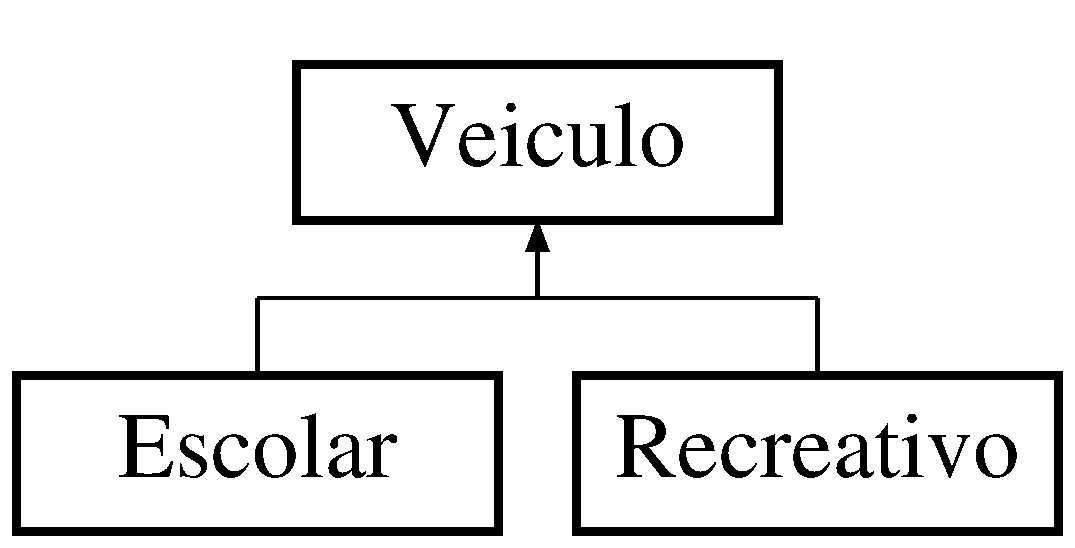
\includegraphics[height=2.000000cm]{class_veiculo}
\end{center}
\end{figure}
\subsection*{Public Member Functions}
\begin{DoxyCompactItemize}
\item 
\mbox{\hyperlink{class_veiculo_a49f6527e767c1ca17a56c84729563ade}{Veiculo}} (const string \&\mbox{\hyperlink{class_veiculo_ad9cd698bf39e90508cd0700ee3b9d90b}{matricula}}, float \mbox{\hyperlink{class_veiculo_a06533b15de432c2d6ee86057d35dc547}{consumo100km}}, float \mbox{\hyperlink{class_veiculo_a1b3f7e8c716e8fd68ec7c7405f18c1ef}{preco\+Comb}})
\begin{DoxyCompactList}\small\item\em Construtor da classe \mbox{\hyperlink{class_veiculo}{Veiculo}}. \end{DoxyCompactList}\item 
unsigned int \mbox{\hyperlink{class_veiculo_aeb0746b1f86094cd9b5689c8c83af98d}{get\+Id}} () const
\begin{DoxyCompactList}\small\item\em Permite acesso ao identificador interno do veiculo. \end{DoxyCompactList}\item 
string \mbox{\hyperlink{class_veiculo_ac41e88b8567d6fca2e932d2df3fd23b5}{get\+Matricula}} () const
\begin{DoxyCompactList}\small\item\em Permite acesso a matricula do veiculo. \end{DoxyCompactList}\item 
float \mbox{\hyperlink{class_veiculo_a4d2607bc367820d260103327dfc502f4}{get\+Consumo}} () const
\begin{DoxyCompactList}\small\item\em Permite acesso consumo em Litros por 100 kms do veiculo. \end{DoxyCompactList}\item 
float \mbox{\hyperlink{class_veiculo_a9f553ab3febd3b756643533f065a289a}{get\+Preco}} () const
\begin{DoxyCompactList}\small\item\em Permite acesso ao preco do combustivel usado no veiculo. \end{DoxyCompactList}\item 
\mbox{\Hypertarget{class_veiculo_a45ee157e20f9408b1c184ba0608178ba}\label{class_veiculo_a45ee157e20f9408b1c184ba0608178ba}} 
virtual unsigned int {\bfseries get\+Lugs\+Livres} () const
\item 
\mbox{\Hypertarget{class_veiculo_a0be7cbd0298ea47a60508f62c899c733}\label{class_veiculo_a0be7cbd0298ea47a60508f62c899c733}} 
virtual vector$<$ unsigned int $>$ {\bfseries get\+Zonas} () const
\item 
\mbox{\Hypertarget{class_veiculo_a8b57e5682a2387a38eb4b8000cc70c18}\label{class_veiculo_a8b57e5682a2387a38eb4b8000cc70c18}} 
virtual void {\bfseries adicionar\+Zona} (unsigned int zona)
\item 
\mbox{\Hypertarget{class_veiculo_ae916bf4719fe50b335a72aea193d3916}\label{class_veiculo_ae916bf4719fe50b335a72aea193d3916}} 
virtual void {\bfseries remover\+Zona} (unsigned int zona)
\item 
\mbox{\Hypertarget{class_veiculo_a964fd208eb010bf1a693247b4ff83acb}\label{class_veiculo_a964fd208eb010bf1a693247b4ff83acb}} 
virtual bool {\bfseries get\+Estado} () const
\item 
\mbox{\Hypertarget{class_veiculo_ad8e27ab7a739537280787e8b47c6e317}\label{class_veiculo_ad8e27ab7a739537280787e8b47c6e317}} 
virtual void {\bfseries set\+Estado} (bool alugado)
\item 
\mbox{\Hypertarget{class_veiculo_aa0828192f9821ff9e319cc7b26729e9e}\label{class_veiculo_aa0828192f9821ff9e319cc7b26729e9e}} 
virtual unsigned int {\bfseries get\+Capacidade} () const
\item 
\mbox{\Hypertarget{class_veiculo_aa3061935859118b6364559d48aa5d3ae}\label{class_veiculo_aa3061935859118b6364559d48aa5d3ae}} 
virtual bool {\bfseries existe\+Zona} (unsigned int zona)
\item 
\mbox{\Hypertarget{class_veiculo_ad256b27a0674b084cdf1e26a019ffedc}\label{class_veiculo_ad256b27a0674b084cdf1e26a019ffedc}} 
virtual float {\bfseries calc\+Gasto} (float kms) const =0
\item 
\mbox{\Hypertarget{class_veiculo_a185fc0670609d87e415e849ed5b6f528}\label{class_veiculo_a185fc0670609d87e415e849ed5b6f528}} 
virtual bool {\bfseries cheio} () const
\item 
\mbox{\Hypertarget{class_veiculo_a9b7aca616ed9b33fc6b0d62f63765013}\label{class_veiculo_a9b7aca616ed9b33fc6b0d62f63765013}} 
virtual void {\bfseries aumenta\+Lug} ()
\item 
\mbox{\Hypertarget{class_veiculo_a9ffe3fdff35855b37350fbd75530b305}\label{class_veiculo_a9ffe3fdff35855b37350fbd75530b305}} 
virtual void {\bfseries reduz\+Lug} ()
\item 
virtual string \mbox{\hyperlink{class_veiculo_a37cf6866bac6b2e7e8837237ec293d48}{get\+Info}} () const
\begin{DoxyCompactList}\small\item\em Organiza a informacao do veiculo para ser guardada em ficheiro. \end{DoxyCompactList}\end{DoxyCompactItemize}
\subsection*{Static Public Attributes}
\begin{DoxyCompactItemize}
\item 
\mbox{\Hypertarget{class_veiculo_a5f4ef3639e6968b83bd3eee911168de4}\label{class_veiculo_a5f4ef3639e6968b83bd3eee911168de4}} 
static unsigned int \mbox{\hyperlink{class_veiculo_a5f4ef3639e6968b83bd3eee911168de4}{num\+Veiculos}} = 0
\begin{DoxyCompactList}\small\item\em Membro estatico que guarda qual o numero de identificacao do ultimo veiculo registado. \end{DoxyCompactList}\end{DoxyCompactItemize}
\subsection*{Protected Attributes}
\begin{DoxyCompactItemize}
\item 
\mbox{\Hypertarget{class_veiculo_a62ec1732abcd9b6eb6a1bc80b6f28ead}\label{class_veiculo_a62ec1732abcd9b6eb6a1bc80b6f28ead}} 
const unsigned int \mbox{\hyperlink{class_veiculo_a62ec1732abcd9b6eb6a1bc80b6f28ead}{idV}}
\begin{DoxyCompactList}\small\item\em Identificacao interna do veiculo. \end{DoxyCompactList}\item 
\mbox{\Hypertarget{class_veiculo_ad9cd698bf39e90508cd0700ee3b9d90b}\label{class_veiculo_ad9cd698bf39e90508cd0700ee3b9d90b}} 
const string \mbox{\hyperlink{class_veiculo_ad9cd698bf39e90508cd0700ee3b9d90b}{matricula}}
\begin{DoxyCompactList}\small\item\em Matricula do veiculo (Nota\+: nao ha matriculas repetidas) \end{DoxyCompactList}\item 
\mbox{\Hypertarget{class_veiculo_a06533b15de432c2d6ee86057d35dc547}\label{class_veiculo_a06533b15de432c2d6ee86057d35dc547}} 
float \mbox{\hyperlink{class_veiculo_a06533b15de432c2d6ee86057d35dc547}{consumo100km}}
\begin{DoxyCompactList}\small\item\em Volume medio de Litros consumidos por 100 kms. \end{DoxyCompactList}\item 
\mbox{\Hypertarget{class_veiculo_a1b3f7e8c716e8fd68ec7c7405f18c1ef}\label{class_veiculo_a1b3f7e8c716e8fd68ec7c7405f18c1ef}} 
float \mbox{\hyperlink{class_veiculo_a1b3f7e8c716e8fd68ec7c7405f18c1ef}{preco\+Comb}}
\begin{DoxyCompactList}\small\item\em Preco do combustivel usado no veiculo. \end{DoxyCompactList}\end{DoxyCompactItemize}
\subsection*{Friends}
\begin{DoxyCompactItemize}
\item 
\mbox{\Hypertarget{class_veiculo_ae5cee715fe9d5928eb95e7d3e5aef756}\label{class_veiculo_ae5cee715fe9d5928eb95e7d3e5aef756}} 
ostream \& {\bfseries operator$<$$<$} (ostream \&out, const \mbox{\hyperlink{class_veiculo}{Veiculo}} \&veic)
\end{DoxyCompactItemize}


\subsection{Detailed Description}
Classe para instanciar veiculos. 

Esta classe agrupa todas as caracteristicas de um veiculo. Permite definir os tracos gerais de um veiculo usado pela \mbox{\hyperlink{class_empresa}{Empresa}}, i.\+e. matricula, identificacao, consumo e preco de combustivel. Com base nesta classe e nas suas derivadas (\mbox{\hyperlink{class_escolar}{Escolar}} e \mbox{\hyperlink{class_recreativo}{Recreativo}}) e possivel executar operacoes como alugar um transporte recreativo, calcular o gasto no percurso efetuado, definir as zonas por onde o transporte escolar passa, etc. 

\subsection{Constructor \& Destructor Documentation}
\mbox{\Hypertarget{class_veiculo_a49f6527e767c1ca17a56c84729563ade}\label{class_veiculo_a49f6527e767c1ca17a56c84729563ade}} 
\index{Veiculo@{Veiculo}!Veiculo@{Veiculo}}
\index{Veiculo@{Veiculo}!Veiculo@{Veiculo}}
\subsubsection{\texorpdfstring{Veiculo()}{Veiculo()}}
{\footnotesize\ttfamily Veiculo\+::\+Veiculo (\begin{DoxyParamCaption}\item[{const string \&}]{matricula,  }\item[{float}]{consumo100km,  }\item[{float}]{preco\+Comb }\end{DoxyParamCaption})}



Construtor da classe \mbox{\hyperlink{class_veiculo}{Veiculo}}. 


\begin{DoxyParams}{Parameters}
{\em matricula} & Matricula do veiculo \\
\hline
{\em consumo100km} & Consumo em Litros por cada 100 kms \\
\hline
{\em preco\+Comb} & Preco do combustivel usado no veiculo \\
\hline
\end{DoxyParams}


\subsection{Member Function Documentation}
\mbox{\Hypertarget{class_veiculo_a4d2607bc367820d260103327dfc502f4}\label{class_veiculo_a4d2607bc367820d260103327dfc502f4}} 
\index{Veiculo@{Veiculo}!get\+Consumo@{get\+Consumo}}
\index{get\+Consumo@{get\+Consumo}!Veiculo@{Veiculo}}
\subsubsection{\texorpdfstring{get\+Consumo()}{getConsumo()}}
{\footnotesize\ttfamily float Veiculo\+::get\+Consumo (\begin{DoxyParamCaption}{ }\end{DoxyParamCaption}) const}



Permite acesso consumo em Litros por 100 kms do veiculo. 

\begin{DoxyReturn}{Returns}
consumo100km do veiculo 
\end{DoxyReturn}
\mbox{\Hypertarget{class_veiculo_aeb0746b1f86094cd9b5689c8c83af98d}\label{class_veiculo_aeb0746b1f86094cd9b5689c8c83af98d}} 
\index{Veiculo@{Veiculo}!get\+Id@{get\+Id}}
\index{get\+Id@{get\+Id}!Veiculo@{Veiculo}}
\subsubsection{\texorpdfstring{get\+Id()}{getId()}}
{\footnotesize\ttfamily unsigned int Veiculo\+::get\+Id (\begin{DoxyParamCaption}{ }\end{DoxyParamCaption}) const}



Permite acesso ao identificador interno do veiculo. 

\begin{DoxyReturn}{Returns}
identificacao do veiculo 
\end{DoxyReturn}
\mbox{\Hypertarget{class_veiculo_a37cf6866bac6b2e7e8837237ec293d48}\label{class_veiculo_a37cf6866bac6b2e7e8837237ec293d48}} 
\index{Veiculo@{Veiculo}!get\+Info@{get\+Info}}
\index{get\+Info@{get\+Info}!Veiculo@{Veiculo}}
\subsubsection{\texorpdfstring{get\+Info()}{getInfo()}}
{\footnotesize\ttfamily string Veiculo\+::get\+Info (\begin{DoxyParamCaption}{ }\end{DoxyParamCaption}) const\hspace{0.3cm}{\ttfamily [virtual]}}



Organiza a informacao do veiculo para ser guardada em ficheiro. 

\begin{DoxyReturn}{Returns}
string com toda a informacao do veiculo (atributos separados por tabs) 
\end{DoxyReturn}


Reimplemented in \mbox{\hyperlink{class_recreativo_a594c854bbcb834cff82c0687afa2b9ce}{Recreativo}}, and \mbox{\hyperlink{class_escolar_aa1f8528c1457656ba5772a253c51b872}{Escolar}}.

\mbox{\Hypertarget{class_veiculo_ac41e88b8567d6fca2e932d2df3fd23b5}\label{class_veiculo_ac41e88b8567d6fca2e932d2df3fd23b5}} 
\index{Veiculo@{Veiculo}!get\+Matricula@{get\+Matricula}}
\index{get\+Matricula@{get\+Matricula}!Veiculo@{Veiculo}}
\subsubsection{\texorpdfstring{get\+Matricula()}{getMatricula()}}
{\footnotesize\ttfamily string Veiculo\+::get\+Matricula (\begin{DoxyParamCaption}{ }\end{DoxyParamCaption}) const}



Permite acesso a matricula do veiculo. 

\begin{DoxyReturn}{Returns}
matricula do veiculo 
\end{DoxyReturn}
\mbox{\Hypertarget{class_veiculo_a9f553ab3febd3b756643533f065a289a}\label{class_veiculo_a9f553ab3febd3b756643533f065a289a}} 
\index{Veiculo@{Veiculo}!get\+Preco@{get\+Preco}}
\index{get\+Preco@{get\+Preco}!Veiculo@{Veiculo}}
\subsubsection{\texorpdfstring{get\+Preco()}{getPreco()}}
{\footnotesize\ttfamily float Veiculo\+::get\+Preco (\begin{DoxyParamCaption}{ }\end{DoxyParamCaption}) const}



Permite acesso ao preco do combustivel usado no veiculo. 

\begin{DoxyReturn}{Returns}
preco do combustivel do veiculo 
\end{DoxyReturn}


The documentation for this class was generated from the following files\+:\begin{DoxyCompactItemize}
\item 
C\+:/\+Users/\+Cajo/\+Desktop/\+Repos/\+A\+E\+D\+A-\/\+P\+R\+O\+J1/src/Veiculo.\+h\item 
C\+:/\+Users/\+Cajo/\+Desktop/\+Repos/\+A\+E\+D\+A-\/\+P\+R\+O\+J1/src/Veiculo.\+cpp\end{DoxyCompactItemize}

%--- End generated contents ---

% Index
\backmatter
\newpage
\phantomsection
\clearemptydoublepage
\addcontentsline{toc}{chapter}{Index}
\printindex

\end{document}
